% Document setup
\documentclass[11pt]{book}

% Location of the csas-style repository: adjust path as needed
\newcommand{\locRepo}{csas-style}

% Use the style file in the csas-style repository (sr.sty)
\usepackage{\locRepo/sr-french}

% header-includes from R markdown entry
\usepackage{pdflscape}
\newcommand{\blandscape}{\begin{landscape}}
\newcommand{\elandscape}{\end{landscape}}
\newcommand{\beginAppA}{ \setcounter{table}{0}\renewcommand{\thetable}{A\arabic{table}}\setcounter{figure}{0}\renewcommand{\thefigure}{A\arabic{figure}} }

%%%% Commands for title page etc %%%%%

% Title
\newcommand{\rdTitle}{Évaluation de la robustesse des procédures de gestion proposées pour la pêche à la morue charbonnière (\emph{Anoplopoma fimbria}) en C.-B., 2019-2020}

% English title
\newcommand{\rdTitleFr}{Evaluating the robustness of candidate management procedures in the BC sablefish (\emph{Anoplopoma fibria}) fishery for 2019-2020.}

% Title short
\newcommand{\rdTitleShort}{Robustesse des PG de la morue charbonnière en C.-B.}
% End of title short

% Publication year
\newcommand{\rdYear}{2019}

% Publication month
\newcommand{\rdMonth}{Novembre}

% Report number
\newcommand{\rdNumber}{\threedigits{999}}
% End of report number

% Approver (name\\position)
\newcommand{\rdApp}{Carmel Lowe\\
Directeur régional}

% Approval date
\newcommand{\rdAppDate}{4 Novembre 2019}

% Branch
\newcommand{\rdBranch}{Secteur des sciences}

% Region
\newcommand{\rdRegion}{Région du Pacifique}

%%%% End of title page commands %%%%%

%Defines cslreferences environment
%Required by pandoc 2.8
%Copied from https://github.com/rstudio/rmarkdown/issues/1649

\DeclareGraphicsExtensions{.png,.pdf}
\begin{document}

\bookmark[dest=PageOne]{\rdTitle{}}

\renewcommand{\tablename}{Tableau}

\MakeFirstPage

\hypertarget{contexte}{%
\section{Contexte}\label{contexte}}

Depuis 2008, Pêches et Océans Canada (MPO) et l'industrie de la pêche du poisson de fond en Colombie-Britannique collaborent à un processus d'évaluation des stratégies de gestion qui vise à maintenir une stratégie transparente et durable de pêche de la morue charbonnière dans la province. La transparence et la durabilité éventuelle des procédures de gestion proposées sont déterminées par des simulations qui mesurent ces procédures par rapport aux objectifs en matière de biologie et de pêche approuvés au préalable. Les modèles d'exploitation sur lesquels reposent les simulations visent à représenter les principales incertitudes liées à l'état des stocks de morue charbonnière et à la productivité. Le processus d'évaluation des stratégies de gestion de la morue charbonnière a fait l'objet de plusieurs examens par les pairs du Secrétariat canadien de consultation scientifique (SCCS) et de publications scientifiques indépendantes évaluées par les pairs (Cox and Kronlund \protect\hyperlink{ref-cox2008practical}{2008}; Cox et al. \protect\hyperlink{ref-cox2011management}{2011}, \protect\hyperlink{ref-cox2013roles}{2013}, \protect\hyperlink{ref-cox2019evaluating}{2019}; DFO \protect\hyperlink{ref-dfo2014performanc}{2014}). Depuis 2011, le MPO publie chaque année des avis sur la pêche canadienne de la morue charbonnière en fonction des simulations des procédures de gestion.

Le processus d'évaluation des stratégies de gestion de la morue charbonnière s'effectue tous les trois ans. Il permet de rajuster le modèle d'exploitation selon les dernières données sur les indices de la biomasse fondés sur les relevés et la pêche, les prises selon l'âge, les remises à l'eau, l'étiquetage et la recapture des poissons étiquetés. Chaque mise à jour triennale offre également l'occasion de modifier les objectifs de pêche et de proposer de nouvelles procédures de gestion.

Les évaluations antérieures de la morue charbonnière en Colombie-Britannique et les travaux en matière d'évaluation des stratégies de gestion ont démontré que le faible recrutement (en moyenne) au cours des trois dernières décennies a contribué au déclin à long terme de la biomasse du stock reproducteur et des possibilités de récolte. Les consultations auprès des intervenants et des gestionnaires ont révélé que la mortalité des poissons de taille inférieure à la taille réglementaire qui sont remis à l'eau (c.-à-d. les poissons de moins de 55 cm) pouvait être une source de mortalité dont la réduction ou l'évitement pourrait améliorer la production de morues charbonnières de plus de 55 cm, la biomasse du stock reproducteur et, finalement, les possibilités de récolte futures (Cox et al. \protect\hyperlink{ref-cox2019evaluating}{2019}). Bien que le processus d'évaluation de la stratégie de gestion de la morue charbonnière ait mentionné certaines mesures volontaires visant à réduire la mortalité des individus de petite taille (p.~ex. une meilleure communication entre les flottilles et une surveillance électronique accrue), il n'a pas évalué officiellement les mesures de gestion visant à réduire la mortalité de ce type d'individus. Toutefois, les simulations antérieures en boucle fermée laissent supposer que l'évitement complet et la conservation complète des morues charbonnières de petite taille pourraient améliorer la production moyenne annuelle de l'espèce dans les pêches dirigées et rehausser la possibilité de rétablissement des stocks à \(B_{RMS}\) (Cox et al. \protect\hyperlink{ref-cox2011management}{2011}, \protect\hyperlink{ref-cox2019evaluating}{2019}). Malheureusement, l'évitement complet n'est peut-être pas possible, surtout dans les pêches au chalut, étant donné que des morues charbonnières de taille inférieure à la taille réglementaire y sont capturées pendant la pêche d'autres espèces. La conservation complète peut entraîner la perte de possibilités de pêche (particulièrement pour le secteur des pêches au chalut) et une rentabilité moindre pour les pêches dirigées, car les morues charbonnières de taille inférieure à la taille réglementaire valent moins par kilogramme que le poisson de taille réglementaire. Au cours des consultations, les intervenants de l'industrie ont indiqué qu'une solution possible consisterait à offrir des mesures incitant les pêcheurs à modifier leur comportement et à éviter davantage de pêcher des morues charbonnières de taille inférieure.

La Direction générale de la gestion des pêches du MPO a donc demandé à la Direction générale des sciences i) de mettre à jour le modèle d'exploitation de la morue charbonnière pour y inclure les données les plus récentes disponibles (jusqu'en 2018); ii) de mettre à jour les avis sur le rendement escompté de la procédure de gestion actuelle; et iii) d'évaluer d'autres procédures ou mesures de gestion ayant pour but de réduire les pertes de productivité en raison de la mortalité des individus de taille inférieure à la taille réglementaire. La question clé en iii) est de déterminer les procédures de gestion qui réduisent au minimum l'effet de telles mesures sur les possibilités de pêche dans le cadre des pêches non dirigées (c.-à-d. les pêches au chalut) où la morue charbonnière de taille inférieure est capturée accidentellement.

Les avis découlant de la présente réponse des Sciences du SCCS serviront à choisir une nouvelle procédure de gestion de la morue charbonnière pour 2020-2022, procédure qui sera conforme au Cadre pour la pêche durable du MPO et au Cadre décisionnel pour les pêches intégrant l'approche de précaution (MPO \protect\hyperlink{ref-DFO2009}{2009}). De plus, la présente réponse des Sciences informe les gestionnaires des pêches et les intervenants des répercussions, sur le secteur des pêches, de l'atténuation des pertes de productivité en raison des remises à l'eau de morues charbonnières de taille inférieure à la taille réglementaire.

La présente réponse des Sciences découle du processus de réponse des Sciences du 23 septembre 2019 sur l'Évaluation de la performance de la stratégie de gestion alternative de la morue charbonnière en Colombie-Britannique, Canada.

\hypertarget{analyse-et-ruxe9ponse}{%
\section{Analyse et réponse}\label{analyse-et-ruxe9ponse}}

La présente réponse des Sciences a adopté une approche de simulation en boucle fermée pour évaluer le rendement relatif des procédures de gestion proposées pour la pêche de la morue charbonnière en Colombie Britannique, et a eu recours à une méthodologie identique à celle présentée dans le cycle précédent de l'évaluation des stratégies de gestion (Cox et al. \protect\hyperlink{ref-cox2019evaluating}{2019}). Les sous-sections qui suivent décrivent brièvement les données mises à jour qui ont servi à façonner le modèle d'exploitation de la morue charbonnière, les changements requis en fonction de ces données, et les nouveaux éléments de la procédure de gestion qui ont été mis à l'essai. D'autres détails sur les mécanismes de simulation, les vérifications diagnostiques et les calculs des mesures du rendement peuvent être consultés dans Cox et al. (\protect\hyperlink{ref-cox2019evaluating}{2019}).

La présente réponse des Sciences a pour but de :
\begin{enumerate}
\def\labelenumi{\arabic{enumi}.}

\item
  décrire les ajustements et les inférences du modèle d'exploitation après sa modification en fonction des indices de biomasse à jour, des prises selon l'âge, et des nouvelles données sur les prises selon l'âge tirées de l'échantillonnage de la morue charbonnière pour déterminer sa composition selon la longueur dans la pêche au chalut;
\item
  établir à partir de ces données une grille de cinq modèles d'exploitation de référence et de cinq modèles de robustesse fondés sur les incertitudes associées à l'état et à la productivité des stocks de morue charbonnière (modèles d'exploitation de référence) et sur le recrutement pour l'année 2015 (modèles d'exploitation de robustesse);
\item
  mener des exercices de simulation des procédures de gestion proposées dans le cadre des modèles d'exploitation de référence et de robustesse en fonction du rendement par rapport aux objectifs de pêche (voir ci-dessous), et classer les procédures de gestion.
\end{enumerate}
\hypertarget{muxe9thodes}{%
\subsection{Méthodes}\label{muxe9thodes}}

\hypertarget{mise-uxe0-jour-du-moduxe8le-dexploitation}{%
\subsubsection{Mise à jour du modèle d'exploitation}\label{mise-uxe0-jour-du-moduxe8le-dexploitation}}

Les données mises à jour jusqu'en 2018 comprenaient les indices de biomasse et les prises selon l'âge découlant du relevé aléatoire stratifié au casier, les prises selon l'âge pour la pêche commerciale au casier, ainsi que les prises et les remises à l'eau totales (en unités de biomasse) pour la pêche commerciale au casier, à la palangre et au chalut. Nous avons également obtenu de nouveaux ensembles de données sur les prises selon l'âge et selon la longueur pour la pêche au chalut afin d'aider à estimer la sélectivité des chaluts, qui est le déterminant clé des prises de morues charbonnières de taille inférieure à la taille réglementaire dans les pêches au chalut. L'ensemble complet des données sur les prises selon l'âge dans les pêches au chalut (avec quelques années manquantes) est fondé sur une clé âge-longueur créée à partir des données sur l'âge et la longueur recueillies de 1972 à 2017.

Le modèle d'exploitation a fait l'objet de légers changements dans le cadre des exercices réguliers visant à accroître l'harmonisation avec diverses données. Mentionnons entre autres i) la modification de la forme fonctionnelle de la sélectivité des chaluts à une fonction de densité gamma (figure A5); ii) la baisse de l'âge 3 à l'âge 2 pour la classe d'âge la plus jeune dans toutes les séries de composition d'âge afin de refléter la gamme des observations âge composition; iii) l'ajout de nouvelles données âge-composition pour la pêche au chalut (annexe A); iv) l'ajout d'un écart estimé du recrutement en 2015 au lieu de l'utilisation du recrutement escompté à partir de la courbe stock-recrutement; v) la mise à jour de la matrice des erreurs de détermination de l'âge afin d'utiliser une approximation normale plus simple, comme recommandé dans l'examen précédent du SCCS (Cox et al. \protect\hyperlink{ref-cox2019evaluating}{2019}); et vi) l'imposition d'un écart-type de \(\sigma = 0,1\) (sur l'échelle logarithmique) aux erreurs d'observation relatives aux remises à l'eau dans le cadre de la pêche au chalut afin d'obtenir une meilleure correspondance à ces données. Les modèles précédents évitaient d'estimer le recrutement au cours des trois années précédentes, surtout parce que cette pratique aurait fourni les premières observations âge-mise à l'eau aux fins du modèle d'exploitation. De plus, il existe en général peu de renseignements pour justifier ces estimations étant donné que les poissons sont trop petits pour être sélectionnés par les pêches ou les relevés. Toutefois, aux fins de la présente mise à jour, le changement décrit en iv) ci-dessus a été retenu (c.-à-d. l'écart de recrutement estimé en 2015) parce qu'il fallait améliorer les correspondances avec les récentes observations de remises à l'eau (très élevées) dans les pêches au chalut. Autrement, nous simulerions les effets des remises à l'eau à partir d'un modèle qui ne correspond pas adéquatement aux remises à l'eau historiques. Ce changement pourrait avoir une incidence importante sur le rendement simulé de la procédure de gestion et, par conséquent, constitue le point central des modèles d'exploitation de robustesse (décrits ci dessous).

\hypertarget{moduxe8les-dexploitation-examinuxe9s}{%
\subsubsection{Modèles d'exploitation examinés}\label{moduxe8les-dexploitation-examinuxe9s}}

\hypertarget{moduxe8les-dexploitation-de-ruxe9fuxe9rence}{%
\subsubsection{Modèles d'exploitation de référence}\label{moduxe8les-dexploitation-de-ruxe9fuxe9rence}}

Les modèles d'exploitation de référence ont été établis à l'aide de la même méthode que celle utilisée pour le cycle précédent de l'évaluation des stratégies de gestion (Cox et al. \protect\hyperlink{ref-cox2019evaluating}{2019}). En résumé, les cinq modèles d'exploitation ont été créés en fonction de la répartition conjointe a posteriori de la biomasse du stock reproducteur de 2018 (pour représenter le risque biologique à court terme) et de l'inclinaison de la pente de la relation stock-recrutement (pour représenter le risque de productivité à long terme des stocks). Les cinq combinaisons ont été choisies pour représenter la moyenne marginale conjointe de la biomasse et de l'inclinaison en 2018 et quatre points extérieurs à l'intersection de la moyenne d'une variable, ainsi que les 10e et 90e centiles de la densité marginale de l'autre variable (figure 1). Cet ensemble de cinq modèles d'exploitation a été choisi pour assurer la cohérence avec le cycle précédent de l'évaluation des stratégies de gestion (Cox et al. \protect\hyperlink{ref-cox2019evaluating}{2019}). Pour chacun des cinq points a posteriori, le modèle d'exploitation a été façonné par un échantillon de 100 sélections a posteriori devant se situer selon une distance de Mahalanobis à 0,75 unité par rapport à ce point. Une estimation empirique de la densité a posteriori a ensuite été appliquée à chacun des cinq centres comme cote de probabilité pour la pondération du rendement de la procédure de gestion, aux fins des cinq modèles d'exploitation pour chacun des ensembles de référence et de robustesse.

\hypertarget{moduxe8les-dexploitation-de-robustesse}{%
\subsubsection{Modèles d'exploitation de robustesse}\label{moduxe8les-dexploitation-de-robustesse}}

Les modèles d'exploitation de robustesse étaient identiques aux cinq modèles d'exploitation de référence, sauf en ce qui concerne la façon dont le recrutement pour la classe de 2015 était traité dans l'élaboration des modèles d'exploitation historiques et les projections. Les modèles d'exploitation de référence utilisés s'inspirent de la répartition conjointe a posteriori (comme elle est définie ci-dessus) pour la classe de 2015. Celle-ci correspond à environ 22 millions de poissons, soit environ 8 fois la moyenne historique. Pour ce qui est des modèles d'exploitation de robustesse, le recrutement a été simulé en fonction de la relation stock-recrutement découlant de la classe 2015 prévue, qui se rapprochait davantage de la moyenne à long terme (\(\sim 2,63\) millions).

\hypertarget{objectifs-de-puxeache}{%
\subsubsection{Objectifs de pêche}\label{objectifs-de-puxeache}}

Les objectifs pour la pêche de la morue charbonnière la Colombie-Britannique ont été mis au point progressivement au cours des dix dernières années grâce à des consultations entre les gestionnaires de pêche, les scientifiques et les intervenants de l'industrie (Cox and Kronlund \protect\hyperlink{ref-cox2009evaluation}{2009}; Cox et al. \protect\hyperlink{ref-cox2011management}{2011}, \protect\hyperlink{ref-cox2019evaluating}{2019}; DFO \protect\hyperlink{ref-dfo2014performanc}{2014}). Les cinq principaux objectifs qui guident cette pêche sont les suivants :
\begin{enumerate}
\def\labelenumi{\arabic{enumi}.}

\item
  \textbf{P(fBSR \textgreater{} PRL)} : Maintenir la biomasse du stock reproducteur femelle (SRF) au-dessus du point de référence limite \(PRL = 0,4B_{RMS}\), où \(B_{RMS}\) représente le modèle d'exploitation de la biomasse du stock reproducteur femelle équivalant à un rendement maximal durable (\(RMS\)), pour 95 \% des années mesurées sur deux générations de morues charbonnières (36 ans).
\item
  \textbf{P(déclin)} : Lorsque la biomasse du stock reproducteur femelle se situe entre \(0,4B_{RMS}\) et \(0,8B_{RMS}\), limiter la probabilité d'un déclin au cours des 10 prochaines années d'un taux très faible (5 \%) de \(0,4B_{RMS}\) à un taux modéré (50 \%) de \(0,8B_{RMS}\). À des niveaux intermédiaires de l'état du stock, définir la tolérance au déclin par une polarisation linéaire entre ces probabilités.
\item
  \textbf{P(fBSR \textgreater{} B\_\(B_{RMS}\))} : Maintenir la biomasse du stock reproducteur femelle au-dessus du niveau cible de a) \(B_{RMS}\) à l'intérieur de la zone saine, ou de b) \(0,8B_{RMS}\) au moment du rétablissement de la zone de prudence en 2052, avec une probabilité de 50 \%.
\item
  \textbf{P(TAC \textless{} 1 992 t)} : Réduire le plus possible la probabilité que les niveaux annuels du total autorisé des captures (TAC) soient inférieurs à 1 992 tonnes pendant deux générations de morue charbonnière.
\item
  \textbf{Prises maximales} : Optimiser les prises annuelles moyennes sur 10 ans, sous réserve des objectifs 1 à 4.
\end{enumerate}
Les mesures de rendement correspondant aux objectifs de pêche 1 à 4 (en gras) s'expriment en tant que « probabilité de (condition) ». Les mesures de rendement sont calculées pour chaque reproduction de simulation, et le rendement escompté pour une procédure de gestion est résumé par la moyenne (ou la médiane) des 100 reproductions de chaque simulation. Les détails complets des mesures de rendement et des calculs sont présentés dans Cox et al. (\protect\hyperlink{ref-cox2019evaluating}{2019}).

Tel qu'il a été mentionné précédemment, il y a une bonification de prix pour les classes de morues charbonnières de plus grande taille, ce qui signifie que le même tonnage de prises débarquées peut donner des valeurs très différentes à quai si les répartitions sous-jacentes des poissons selon la taille varient grandement. Cette situation peut avoir des conséquences sur les mesures de gestion des individus de taille inférieure à la taille réglementaire, qui exigent le débarquement de petites morues charbonnières (sans limite de taille). Par conséquent, en plus de présenter des statistiques sur le rendement des prises (objectif de pêche 5), l'évaluation a calculé les recettes cumulatives sur 10 ans et le revenu moyen par tonne pour chaque flottille (parce que la composition des prises en fonction des tailles varie également selon la flottille).

\hypertarget{procuxe9dures-de-gestion}{%
\subsubsection{Procédures de gestion}\label{procuxe9dures-de-gestion}}

Une procédure de gestion s'entend d'un algorithme précis et reproductible servant à calculer le total autorisé des captures (TAC) annuel pour une catégorie de pêche. Dans la plupart des cas, les procédures de gestion comprennent des données de surveillance, des méthodes d'évaluation pour le traitement des données et l'estimation de l'état des stocks, des règles de contrôle de la récolte pour traduire les extrants de l'évaluation en limites de prises, des métarègles qui peuvent inclure des contraintes sur les changements des TAC, ainsi que des conditions (p.~ex. circonstances exceptionnelles) pour déclencher des déviations par rapport à l'avis habituel sur la récolte des procédures de gestion.

La procédure de gestion qui sert actuellement à calculer le TAC pour la morue charbonnière a été établie pour la première fois en 2011, puis modifiée à l'occasion des deux versions subséquentes de l'évaluation des stratégies de gestion. En général, la procédure de gestion inclut i) des \textbf{données} -- prises débarquées et trois indices de la biomasse; ii) une \textbf{méthode d'évaluation} -- un modèle de production excédentaire comportant des erreurs d'observation et de processus afin d'estimer la biomasse du stock à partir des indices de la biomasse et des prises débarquées; iii) un \textbf{rapport de contrôle de la récolte} -- un rapport 60:40 au titre du contrôle de la récolte selon lequel le taux de récolte cible est rajusté à partir de 0 \% lorsque la biomasse estimée est inférieure à 40 \% de \(B_{RMS}\) à une valeur maximale lorsque la biomasse estimée est supérieure à 60 \% de la valeur \(B_{RMS}\) estimée; iv) une \textbf{métarègle} -- précisant que les hausses du TAC sont nulles à moins que le rapport de contrôle de la récolte recommande une augmentation de plus de 200 tonnes (les diminutions du TAC sont toujours adoptées); et v) une \textbf{métarègle} -- ramenant le taux maximal cible de mortalité des poissons de 9,5 \% en 2017 à 5,5 \% en 2021. Les TAC sont répartis entre les trois secteurs ainsi : 40,37 \% pour le casier, 50,90 \% pour la palangre et 8,75 \% pour le chalut; les quotas restants sont réservés aux relevés. La production attribuée à la pêche au chalut découle de négociations entre les secteurs qui ont fixé l'attribution des prises en fonction des évaluations précédentes des stratégies de gestion (Cox et al. \protect\hyperlink{ref-cox2011management}{2011}), tandis que les prises allouées à la pêche à la palangre et à celle au chalut sont calculées en fonction de la part moyenne des prises dans chaque secteur au cours de la période de 2009 à 2018.

La présente réponse des Sciences repose sur l'évaluation du rendement de la procédure de gestion actuelle pour la morue charbonnière, un scénario de référence où la population n'est pas exploitée, et 15 versions de la procédure actuelle où seules les mesures de gestion des remises à l'eau varient. Les versions de la procédure de gestion sont établies par la combinaison de trois éléments :
\begin{enumerate}
\def\labelenumi{\arabic{enumi}.}

\item
  le \textbf{plafond de remises à l'eau des poissons de taille inférieure à la taille réglementaire}, qui prévoit que toutes les remises à l'eau sous le plafond peuvent être relâchées sans pénalité et que le nombre de prises excédant le plafond est classé dans les excédents. Les valeurs de plafond sont les suivantes : aucun plafond, 0 \%, 50 \%, 100 \% et 150 \% de plus que la moyenne de 464 t de remises à l'eau entre 2006 et 2018. La procédure de gestion actuelle ne comporte aucun plafond (remises à l'eau illimitées sans pénalité), alors que l'option sans limite de taille (\textbf{SLT}) ne permet aucune remise à l'eau (tous les poissons amenés à bord des navires doivent être débarqués et comptés dans le TAC).
\item
  des \textbf{allocations fixes pour les différentes flottilles} (c.-à-d. casier, palangre et chalut) par rapport au plafond des remises à l'eau. Les allocations sont calculées en fonction de la moyenne des parts récentes (rct = \((23 \%, 18 \%, 59 \%)\), 2016-2018) ou historiques (hst = \((30 \%, 37 \%, 33 \%)\), 2006-2018) du total des remises à l'eau annuelles qui ont été attribuées à chaque flottille.
\item
  une \textbf{période d'amortissement } de 5 (am5) ou 10 (am10) ans au cours de laquelle il faut étaler les excédents des remises à l'eau par rapport aux TAC futurs.
\end{enumerate}
Dans la présente réponse des Sciences, les procédures de gestion sont désignées par la combinaison de trois mesures de gestion en mer décrites ci-dessus : PLAFOND\_ALLOCATION\_ AMORTISSEMENT. Par exemple, la procédure de gestion \textbf{cap.5\_hstAl\_am5} comporte un plafond des remises à l'eau totales fixé à 50 \% (0,5) de la moyenne historique (\textbf{cap.5}), une allocation du plafond entre les flottilles fondée sur les parts moyennes historiques qui s'appliquent à chaque flottille (\textbf{hstAl}), et une période d'amortissement de cinq ans pour les excédents de remises à l'eau (\textbf{am5}). Les deux cas spéciaux de cette convention d'affectation des noms sont : la procédure de gestion actuelle (\textbf{sans plafond}), qui ne comporte aucun plafond, et celle sans limite de taille (\textbf{SLT}), qui ne permet aucune remise à l'eau (toutes les prises sont débarquées quelle que soit leur taille). Pour les plafonds de 0 \%, seule la période d'amortissement pour les excédents s'appliquerait (p.~ex. \textbf{cap0\_am5}), et toutes les remises à l'eau seraient comptées comme des excédents.

\hypertarget{un-exemple-pratique-des-mesures-de-gestion-des-remises-uxe0-leau-dans-le-scuxe9nario-cap.5_hstal_am5}{%
\subsubsection{\texorpdfstring{Un exemple pratique des mesures de gestion des remises à l'eau dans le scénario \textbf{cap.5\_hstAl\_am5}}{Un exemple pratique des mesures de gestion des remises à l'eau dans le scénario cap.5\_hstAl\_am5}}\label{un-exemple-pratique-des-mesures-de-gestion-des-remises-uxe0-leau-dans-le-scuxe9nario-cap.5_hstal_am5}}

Pour illustrer comment ont été établies les simulations de mise en œuvre des mesures de gestion des remises à l'eau, la séquence des calculs utilisés pour déterminer les plafonds annuels de remises à l'eau est présentée ci-dessous, de même que leurs effets sur les allocations futures du TAC. Dans les calculs ci-dessous, \(t\) correspond à l'année, \(g\) à la flottille, et \(p(g)\) à la part des remises à l'eau attribuée à la flottille \(g\).
\begin{enumerate}
\def\labelenumi{\arabic{enumi}.}

\item
  Calculer 50 \% du PLAFOND des remises à l'eau par année et par flottille (464 t est la moyenne de 2006 à 2018) : \begin{equation*} 
  CAP(t,g) = 0,5 \cdot 0,464 \cdot p(g). 
  \end{equation*}
\item
  Exécuter la simulation pour l'année t afin d'obtenir les remises à l'eau réelles : \(R(t,g)\).
\item
  Calculer l'excédent \(o(t,g)\) pour l'année en établissant la différence entre les remises à l'eau réelles \(R(t,g)\) et le plafond \(CAP(t,g)\) : \tabularnewline \begin{equation*} 
  o(t,g) = R(t,g) – CAP(t,g).
  \end{equation*}
\item
  Étant donné que la période d'amortissement est de 5 ans, ajouter 1/5e de l'excédent de cette année au cumulatif des excédents \(O(t+k,g)\) de chacune des cinq années qui suivent : \begin{equation*}
  O(t + k,g) = O(t+k,g) + o(t,g)/5, \mbox{ pour } k = 1, ..., 5.    
  \end{equation*}
\item
  Calculer le TAC rajusté pour la morue charbonnière de taille réglementaire qui vaudra pour l'année prochaine en soustrayant le total de l'excédent pour l'année en question du \(TAC’S initial (\)TAC'S fixé par la procédure de gestion avant les mesures de gestion des remises à l'eau) : \begin{equation*}
  TAC(t,g) = TAC'(t,g) – O(t,g).
  \end{equation*}
\end{enumerate}
Cette méthode vise à inciter les pêcheurs à ne pas prendre de morues charbonnières de taille inférieure à la taille réglementaire grâce aux réductions futures du TAC (en supposant un rapprochement un-pour-un de la biomasse des individus de taille inférieure à celle des morues charbonnières de taille réglementaire), tout en permettant une certaine souplesse d'une année à l'autre pour les remises à l'eau importantes et imprévisibles au cours d'une année donnée. Il est à noter que les excédents ne peuvent jamais être inférieurs à zéro, de sorte que les TAC ne peuvent être relevés au-delà du TAC initial établi par la procédure de gestion de premier palier (c.-à-d. qu'il ne peut y avoir de mise en banque des TAC).

\hypertarget{ajustement-des-procuxe9dures-de-gestion}{%
\subsubsection{Ajustement des procédures de gestion}\label{ajustement-des-procuxe9dures-de-gestion}}

L'évaluation de la stratégie de gestion de la morue charbonnière quantifie le rendement des procédures de gestion par rapport aux statistiques sur le rendement qui correspondent à chacun des objectifs de pêche. Les trois premières statistiques sur le rendement sont représentées par le rendement de la conservation de la biomasse par rapport au point de référence limite (PRL), la probabilité d'un déclin à court terme et l'atteinte complète ou partielle d'une cible à long terme de \(B_{RMS}\), tandis que les quatrième et cinquième statistiques ont trait au maintien des niveaux de prises au-dessus d'un plancher privilégié par l'industrie et des prises moyennes à court terme. Il est rare que deux procédures de gestion affichent un rendement comparable pour quatre de ces statistiques de rendement et diffèrent à l'égard d'une seule. Si c'était le cas, la décision sur la procédure de gestion préférée serait simple -- il s'agirait de choisir celle qui affiche le meilleur rendement pour la cinquième statistique. Malheureusement, les procédures de gestion diffèrent généralement sur les cinq statistiques de rendement simultanément, de sorte qu'il est difficile de comparer le rendement sans, à tout le moins, établir une certaine équivalence entre les probabilités de conservation (objectifs de pêche 1 à 3) et les prises moyennes à court terme (objectif de pêche 5).

L'ajustement des procédures de gestion est un moyen d'en établir le rendement équivalent par rapport aux objectifs pour lesquels les valeurs et les probabilités sont bien établies. Par exemple, le maintien du stock de morue charbonnière au-dessus du PRL (\(0,4B_{RMS}\)) avec une forte probabilité n'a pas fait l'objet d'un débat ouvert puisqu'il s'agit d'une directive générale canadienne dans le contexte de la pêche à la morue charbonnière (du moins, il n'y a pas eu de débat au cours des 10 ans et plus d'existence de l'évaluation des stratégies de gestion de la morue charbonnière). De même, le maintien d'une faible probabilité de déclin à court terme n'a pas non plus fait l'objet d'un débat, probablement parce que l'objectif principal de l'industrie de la pêche à la morue charbonnière a été d'éviter un nouveau déclin depuis le début du processus d'évaluation des stratégies de gestion. L'objectif de pêche 3 -- la biomasse du stock reproducteur dans la zone saine d'ici deux générations -- a été débattu au fil des ans pour des raisons pratiques. Plus précisément, on craint que l'atteinte de l'objectif de pêche 3 ne nécessite de sévères restrictions des prises à court terme pour des avantages à long terme très incertains. Au cours de l'année écoulée, l'industrie de la morue charbonnière et le MPO ont convenu de modifier l'objectif de pêche 3 pour obtenir la biomasse dans la zone saine d'ici la fin d'une année précise (2052) avec une probabilité d'au moins 50 \%, c.-à-d. une valeur médiane de la biomasse du stock reproducteur femelle égale ou supérieure à \(B_{RMS}\). Comme nous le démontrons ci-dessous, cet objectif est maintenant réalisable compte tenu de la dynamique de la morue charbonnière et de l'éventail de procédures de gestion réalistes. Toutefois, une nouvelle question se pose à cet égard : Que vaut l'amélioration (c.-à-d. en prises) du rendement au chapitre de l'objectif de pêche 3; par exemple, \(P(B_{2052} \geq B_{MSY}) = 0.5\) to \(P(B_{2052} \geq B_{MSY}) = 0.55\)? Un écart de probabilité de seulement cinq points de pourcentage pourrait signifier une différence de plusieurs centaines de tonnes de prises annuelles moyennes, et des dizaines de millions de dollars en revenus. Les procédures de gestion qui affichent un meilleur rendement relativement à l'objectif de pêche 3 le font presque toujours au détriment du rendement relatif aux objectifs de pêche 4 et 5.

On a tenté de simplifier l'interprétation du rendement des procédures de gestion en les harmonisant toutes avec la formule standard \(P(B_{2052} \geq B_{RMS}) = 0,5\), de sorte que toutes les procédures atteignent les objectifs 1 à 3. Cette harmonisation a été faite par des mises au point progressives de \(F_{2021}\), qui correspond au taux de mortalité maximal de la pêche ciblée pour l'année 2021 (dans le cadre d'une période progressive de 5 ans pour la procédure actuelle) (Cox et al. \protect\hyperlink{ref-cox2019evaluating}{2019}), jusqu'à ce que chaque procédure atteigne l'objectif 3, c.-à-d. \(P(B_{2052} \geq B_{RMS}) = 0,5\). Ces taux cibles de prises maximales \(F_{2021}\) remplacent alors les taux cibles de prises maximales prévus de 5,5 \% pour l'année 2022 et les années suivantes.

Chaque procédure de gestion a été ajustée séparément avec les scénarios des modèles d'exploitation de référence et de robustesse, ce qui a donné des valeurs différentes \(F_{2021}\) (c.-à-d. une pour chaque modèle d'exploitation). Nous avons ensuite simulé un test croisé dans lequel des valeurs \(F_ {2021}\) ajustées selon le modèle d'exploitation de référence ont été appliquées aux procédures de gestion des modèles d'exploitation de robustesse et vice versa. Le test croisé révèle les conséquences biologiques et de capture que peut avoir l'utilisation des mauvaises valeurs \(F_{2021}\).

\hypertarget{ruxe9sultats}{%
\subsection{Résultats}\label{ruxe9sultats}}

\hypertarget{mise-uxe0-jour-du-moduxe8le-dexploitation-et-ruxe9percussions-sur-luxe9tat-des-stocks}{%
\subsubsection{Mise à jour du modèle d'exploitation et répercussions sur l'état des stocks}\label{mise-uxe0-jour-du-moduxe8le-dexploitation-et-ruxe9percussions-sur-luxe9tat-des-stocks}}

Les adaptations du modèle d'exploitation en fonction du relevé et des indices de la biomasse de la pêche étaient semblables à celles des versions précédentes, où le modèle et les données montraient un déclin constant à long terme. Les points de données des deux relevés aléatoires stratifiés les plus récents (2017 et 2018) étaient considérablement plus élevés que ceux des 15 années précédentes, ce qui laisse entrevoir des augmentations éventuelles de la biomasse des stocks extracôtiers (figure 2).

En général, le modèle d'exploitation structuré selon l'âge correspond assez bien aux données sur la composition par âge (figure 3). La composition par âge de la pêche au casier a continué de montrer une importante différence résiduelle positive chez les mâles de 35 ans et plus et, dans une mesure plus négligeable, chez les femelles (figure 3 -- Casier :). La composition par âge de la pêche au chalut a également montré une importante différence résiduelle positive pour les mâles de 2 ans qui semble découler des vastes échantillons de 2017 et de 2018 et, par conséquent, a eu tendance d'entraîner une moyenne qui semble présenter une importante différence résiduelle positive à 2 ans. Il s'agissait d'un élément pouvant déterminer la taille estimative de la classe de l'année 2015.

Le modèle correspondant au relevé normalisé était similaire aux versions précédentes des modèles d'exploitation --- les tendances se situent quelque part entre les ajustements de la composition par âge (pire) et les ajustements du relevé aléatoire stratifié au casier (meilleure) {[}figures 2 et 3{]}. Le modèle d'exploitation continue de très bien correspondre au relevé aléatoire stratifié au casier, probablement parce que celui-ci est conçu spécialement pour surveiller la population extracôtière de morue charbonnière (contrairement à tous les autres ensembles de données).

La mise à jour de l'état des stocks de morue charbonnière canadienne dépendait de la taille absolue de la classe d'âge de 2015 (3 ans au cours de l'année d'évaluation 2018). L'estimation brute de cette classe était d'environ huit fois la moyenne historique (voir la section ci-dessus sur les modèles d'exploitation de robustesse -- figure 4, dernière rangée), ce qui a donné l'impression qu'il s'agissait du plus important recrutement d'une population alors que les biomasses du stock reproducteur étaient à leur plus bas. Un recrutement aussi élevé avec une biomasse du stock reproducteur faible a eu des effets en cascade sur les estimations des paramètres du modèle, les points de référence biologiques et l'estimation de la biomasse actuelle. Ces effets comprenaient : i) la productivité estimative des stocks (c.-à-d. le paramètre d'inclinaison de la pente de la relation stock-recrutement) a été rajustée à la hausse; ii) la taille du stock le plus productif (\(B_{RMS}\)) a été rajustée à la baisse, parce que le stock est semble-t-il plus productif lorsque la biomasse est faible; iii) le taux optimal de mortalité des poissons (\(F_{RMS}\)) a été relevé parce que le stock plus productif peut subir des pressions supérieures sur le plan de la pêche; et iv) la biomasse actuelle du stock reproducteur a été rajustée à la hausse parce qu'environ 20 à 25 \% des poissons âgés de 3 ans arrivaient à maturité. Bien qu'il s'agisse de signes positifs et encourageants qui indiquent que l'état de la morue charbonnière s'améliore, il y avait un certain risque à harmoniser les procédures de gestion futures avec les changements importants apportés au modèle par suite d'un petit nombre d'observations. D'autres pêches de poisson de fond du Pacifique (p.~ex. le merlu du Pacifique {[}\emph{Merluccius productus}{]} et la morue charbonnière du golfe de l'Alaska) ont traité avec circonspection les premières estimations importantes en matière de recrutement tant que les données utilisées pour les estimer ne se matérialiseront pas davantage. Dans le présent cas, l'incertitude quant à la taille des classes de 2015 a été contrée par l'élaboration de modèles d'exploitation de référence (qui utilisent les données relatives à l'âge 3) et de robustesse (qui ne tiennent pas compte des données relatives à l'âge 3) qui serviraient à l'évaluation des procédures de gestion.

En ce qui concerne la grande classe de 2015, le modèle d'exploitation ajusté a révélé que le stock de morue charbonnière était généralement bon (tableau 1, 2018 -- Ajustement). En 2018, la biomasse du stock reproducteur était environ deux fois plus élevée que le point de référence limite (PRL), comparativement à environ 1,5 fois le PRL, qui a lui-même été relevé par rapport à l'ajustement de 2016 qui était d'environ 1,17 fois le PRL. Ce changement indique que les stocks de morue charbonnière de la Colombie-Britannique ne font peut-être plus l'objet d'une surpêche. De même, la probabilité a posteori que la biomasse de l'année précédente soit supérieure au point de référence limite s'est également améliorée de 2016 à 2018, passant de 93 \% (ajustement en 2016) à 100 \% (ajustement en 2018).

\hypertarget{ruxe9sultats-de-luxe9valuation-des-procuxe9dures-de-gestion}{%
\subsubsection{Résultats de l'évaluation des procédures de gestion}\label{ruxe9sultats-de-luxe9valuation-des-procuxe9dures-de-gestion}}

\hypertarget{moduxe8les-dexploitation-de-ruxe9fuxe9rence-uxe9tablis-en-fonction-de-lajustement-f_2021}{%
\subsubsection{\texorpdfstring{Modèles d'exploitation de référence établis en fonction de l'ajustement \(F_{2021}\)}{Modèles d'exploitation de référence établis en fonction de l'ajustement F\_\{2021\}}}\label{moduxe8les-dexploitation-de-ruxe9fuxe9rence-uxe9tablis-en-fonction-de-lajustement-f_2021}}

Comme on s'y attendait, le recrutement de la classe de 2015 a été le principal déterminant de la biomasse estimée du stock reproducteur et des résultats de la pêche projetés dans les simulations du modèle d'exploitation de référence. La biomasse du stock reproducteur s'est accrue rapidement au cours des cinq premières années de la période de prévision (c.-à-d. la classe de 2015), car les poissons âgés de 3 ans ont été entièrement recrutés pour la pêche, puis pour la biomasse du stock recruteur (figures 4 et 5, première rangée). La biomasse du stock recruteur a ensuite connu une tendance à la baisse pour atteindre \(B_{RMS}\) à long terme, car les poissons de la classe de 2015 ont été pêchés et les recrutements sont revenus aux valeurs prévues conformément à la relation stock-recrutement (c.-à-d. les recrutements à partir de 2016 sont tous simulés selon la relation stock-recrutement).

Dans ces conditions, toutes les procédures de gestion respectaient tous les critères biologiques définis dans les objectifs de pêche 1 à 3 (tableau 2). Toutes les procédures de gestion ajustées ont été en mesure d'atteindre l'objectif de pêche 3, alors que la biomasse du stock reproducteur médiane (première rangée de la figure 5) atteindra \(B_{RMS}\) (ligne pointillée horizontale avec des points verts aux extrémités) d'ici la dernière année (2052). Certaines procédures de gestion pourront atteindre \(B_{RMS}\) 15 à 20 ans avant la dernière année, tandis que d'autres arriveront tout juste à réaliser \(B_{RMS}\) la dernière année.

L'ajustement des procédures de gestion (PG) pour qu'elles respectent les objectifs 1 à 3, et plus particulièrement le fait de traiter l'objectif de pêche 3 comme une cible, axent les écarts de rendement des procédures de gestion sur les prises annuelles moyennes au cours des 10 prochaines années (tableau 2 -- Objectif 5). Comme prévu, les procédures de gestion comportant des mesures de gestion des remises à l'eau plus restreintes se sont mieux classées en termes de prises moyennes sur 10 ans (tableau 2), alors que les valeurs variaient de 4 530 t par année pour l'option sans limite de taille (PG17 \textbf{SLT}*) à 3 710 t par année pour les mesures de gestion dont le plafond est supérieur de 150 \% à la moyenne, l'allocation récente du plafond aux diverses flottilles (c.-à-d. l'attribution de 59 \% au chalut) et l'amortissement sur cinq ans (PG14 \textbf{cap1.5\_rctAl\_am5}). Cette différence était attribuable à deux éléments. Tout d'abord, on a adopté comme principale hypothèse que l'activité de pêche cessait une fois que le TAC était atteint, de sorte que la pêche sans limite de taille réduisait la mortalité des poissons de taille inférieure pour l'ensemble des flottilles. Cette hypothèse a mené à une forte réduction de la croissance de la surpêche pour la procédure de gestion sans limite de taille --- les gains relatifs à la croissance de la taille de la morue charbonnière ont été beaucoup plus élevés que les pertes occasionnées par la mortalité naturelle dans les classes de taille inférieure à la taille réglementaire --- et, par conséquent, à un poids moyen des prises de taille réglementaire plus élevé. Deuxièmement, il a été tenu pour acquis que la pêche pourrait s'effectuer à des taux de mortalité plus élevés parce que la survie par rapport aux classes de taille inférieure était plus grande et qu'il y avait donc un plus grand recrutement pour les pêches et le stock reproducteur. En effet, la cible maximale actuelle \(F=5,5\%\)/année apparemment conservatrice des procédures de gestion était en grande partie attribuable à la baisse de la survie dans les classes de taille inférieure à la taille réglementaire, ce qui a empêché les procédures de gestion d'atteindre l'objectif 3 de la pêche sur la biomasse du stock reproducteur. En revanche, la procédure de gestion sans limite de taille a presque atteint l'objectif de pêche 3 malgré une cible maximale de \(F=7,5 \%\)/année pour les poissons de taille réglementaire (tableau 2 -- \(F_{2021}\)).

Les écarts quant aux prises annuelles moyennes étaient plus faibles lorsque les mesures de gestion en mer comportaient une limite de taille. Un plafond de 0 \% pour les remises à l'eau et une période d'amortissement de cinq ans (PG6) ont donné des prises d'environ 400 t de plus que la procédure de gestion actuelle (PG15; tableau 2), alors que le gain était de 300 t pour une période d'amortissement de 10 ans (PG5).

Un plafond des remises à l'eau de 50 \% de la moyenne historique a entraîné des prises annuelles moyennes de 160 t et 300 t de plus que la procédure de gestion actuelle, selon l'allocation et la période d'amortissement (PG3 et PG4 par rapport à PG15; tableau 2). Fait intéressant, un amortissement sur 10 ans avec un plafond de 0 \% produit une prise moyenne sur 10 ans identique à celle fournie par un plafond de 50 \% avec une allocation historique et une période d'amortissement de 5 ans (PG5 par rapport à PG6; tableau 2).

Un plafond de remises à l'eau qui équivaut à 100 \% de la moyenne historique produit également 200 tonnes de prises annuelles moyennes de plus que la procédure de gestion (PG) actuelle, dans la mesure où le plafond a été attribué en fonction des parts historiques de remises à l'eau et amorti sur cinq ans (PG8 par rapport à PG15, tableau 2). La similitude avec le scénario fixant le plafond à 50 \% décrit ci-dessus reflète principalement la part du plafond attribuée à la flottille de chalutiers, où l'allocation récente (59 \%) correspond à près du double de l'allocation historique (33 \%). Par conséquent, en passant à l'allocation inférieure, l'allocation historique a permis de doubler le plafond (c.-à-d. que les montants totaux des remises à l'eau attribués à la flottille de chalutiers étaient semblables). En général, les options d'allocation historique se sont classées plus haut que les allocations récentes parce que l'allocation historique comprend des remises à l'eau plus faibles par la flottille de chalutiers. La période d'amortissement n'a pas eu un effet aussi notable que les options générales de plafonnement et d'allocation, dans cet ordre.

Le relèvement du plafond à 150 \% de la moyenne historique a produit la moyenne annuelle de prises la plus faible, même si la procédure de gestion actuelle n'a aucun plafond (PG13 par rapport à PG15; tableau 2). Bien que les prises moyennes sur 10 ans aient été semblables, les remises à l'eau en vertu de la procédure de gestion actuelle (\textbf{sans plafond}) varient principalement selon le recrutement. Elles ont donc moins d'effet qu'un plafond de 150 \%, qui a dissocié les remises à l'eau et le recrutement dans une faible mesure. Il a aussi permis à la pêche au chalut de continuer d'excéder les taux actuels de prises de taille inférieure à la taille réglementaire.

À mesure que les plafonds étaient relevés en vertu de la récente allocation de remises à l'eau, la meilleure option en matière d'amortissement est passée d'une période de 5 ans (avec des plafonds bas) à 10 ans (avec des plafonds élevés). Bien que les écarts aient été faibles (PG12 par rapport à PG3; tableau 2), cette transition est probablement attribuable au fait qu'il y a peu d'avantages, voire aucun, sur le plan de la surpêche découlant d'un amortissement avec des plafonds élevés et des allocations récentes. Pour la pêche au chalut, cela signifierait des remises à l'eau plus élevées qu'à l'heure actuelle. Dans le cas qui nous occupe, la période d'amortissement a eu un effet direct sur les TAC, alors que les périodes d'amortissement plus longues ont eu moins d'effet parce que les excédents étalés sur une période plus longue jouent moins sur les rajustements annuels des TAC.

Au départ, il semblait qu'une option sans limite de taille ou des mesures de gestion avec un plafond inférieur auraient une incidence négative sur les recettes de la pêche, parce que les prises débarquées comprendraient des proportions plus élevées de poissons de taille inférieure à la taille réglementaire. La bonification des prix pour la morue charbonnière (tableau 3; C. Acheson, communication personnelle, printemps 2019) peut entraîner un écart de plusieurs dollars la livre entre la morue charbonnière de taille inférieure (\textless{} 3 lb) et celle de taille réglementaire (4-5+).

En effet, le revenu moyen par tonne était d'environ 170 \$ inférieur pour une pêche au casier sans limite de taille par rapport à la pêche sans plafond (tableau 4), tandis que les recettes étaient d'environ 20 \$ et 1 070 \$ de moins la tonne pour les prises débarquées par les flottilles de pêche à la palangre et au chalut, respectivement. Les pêches au casier, et surtout les pêches à la palangre, ont opté pour une sélectivité selon la taille se rapprochant suffisamment des plus grandes tailles pour que la conservation des petits poissons ait des conséquences relativement faibles comparativement aux avantages de TAC moyens plus élevés. Les recettes cumulatives sur dix ans ont été de 47 millions de dollars, de 18 millions de dollars et de 15 millions de dollars de plus pour la pêche au casier, à la palangre et au chalut en vertu de la procédure de gestion sans limite de taille, comparativement à la meilleure option suivante du point de vue de la moyenne des prises annuelles (p.~ex. PG6, \textbf{cap0\_am5}; tableau 4).

Les meilleures mesures de gestion des remises à l'eau du point de vue du total des prises et des recettes cumulatives, après l'option sans limite de taille, n'étaient pas les mêmes pour la pêche au casier, à la palangre et au chalut. Par exemple, comme il a été mentionné ci-dessus, la PG6 (\textbf{cap0\_am5}) était la deuxième meilleure option pour les pêches au casier et à la palangre, en termes de TAC annuel moyen et de recettes cumulatives (tableau 4). En revanche, la deuxième meilleure option pour les recettes de la pêche au chalut était la PG14 (\textbf{cap1.5\_rctAl\_am5}), qui avait le TAC annuel moyen le plus bas. La différence au chapitre des recettes pour les pêches au chalut entre cette option et celle sans limite de taille n'était que de 5 millions de dollars sur 10 ans, tandis que l'écart de recettes entre les PG6 et PG17 pour les pêches au casier et à la palangre était de 33 millions de dollars et de 32 millions de dollars, respectivement. Ainsi, les résultats laissent entendre que les pêches au casier et à la palangre bénéficieraient de mesures de gestion en mer plus restrictives, tandis que la pêche au chalut bénéficierait de mesures de gestion en mer moins restrictives que le statu quo, même sans tenir compte des répercussions sur les principales pêches visées par les pêches au chalut.

\hypertarget{moduxe8les-dexploitation-de-robustesse-uxe9tablis-en-fonction-de-lajustement-f_2021}{%
\subsubsection{\texorpdfstring{Modèles d'exploitation de robustesse établis en fonction de l'ajustement \(F_{2021}\)}{Modèles d'exploitation de robustesse établis en fonction de l'ajustement F\_\{2021\}}}\label{moduxe8les-dexploitation-de-robustesse-uxe9tablis-en-fonction-de-lajustement-f_2021}}

Contrairement aux modèles d'exploitation de référence, où les augmentations de la biomasse et des prises sur 10 ans étaient considérables, les estimations concernant la biomasse et les prises de morue charbonnière en vertu des modèles d'exploitation de robustesse ont augmenté plus graduellement, et ont exigé en général des taux de pêche plus faibles pour respecter les objectifs de pêche 1 à 3 (figures 6 et 7). En fait, ces simulations produisent des résultats assez semblables à ceux de l'évaluation précédente des stratégies de gestion de la morue charbonnière, ce qui laisse croire que des stratégies de récolte assez conservatrices s'imposent à long terme pour atteindre les objectifs de pêche 1 à 3 (Cox et al. \protect\hyperlink{ref-cox2019evaluating}{2019}).

Il a été plus difficile de modifier la procédure de gestion afin qu'elle atteigne l'objectif de pêche 3 en vertu des modèles d'exploitation de robustesse, parce que les valeurs \(F\) plus élevées avaient des répercussions plus notables sur l'objectif de déclin à court terme {[}P(déclin); tableau 5{]}. L'ajustement de la procédure de gestion a entraîné des taux de mortalité des poissons assez faibles, qui variaient de 5,2 \% (procédure de gestion actuelle) à 7,2 \% (plafond 0). Ces faibles \(F\) ont également eu pour effet d'accroître la probabilité de prises inférieures à 1 992 t (objectif de pêche 4). Même s'ils étaient négligeables (\textless{} 3 \%) dans les modèles d'exploitation de référence, ils excédaient tous 15 \% dans les modèles d'exploitation de robustesse, sauf pour la procédure de gestion sans limite de taille où ils s'établissaient à 8 \% (tableau 5).

La moyenne des prises annuelles selon les modèles d'exploitation de robustesse variait de 2 305 t selon la procédure de gestion actuelle (PG15, sans plafond) à 2 767 t selon celle sans limite de taille (PG17, sans limite de taille). Par conséquent, la procédure de gestion actuelle, sans limite des remises à l'eau, a affiché un rendement inférieur à celui de n'importe laquelle des options ayant un plafond, et a même produit 200 t de moins par année pour les options avec plafond les mieux classées (tableau 5). Il y avait une légère différence dans l'ordre de classement des procédures de gestion (classées selon la moyenne des prises sur 10 ans) aux termes des modèles d'exploitation de robustesse, comparativement aux modèles d'exploitation de référence, bien que la différence absolue entre la plupart des procédures de gestion soit faible.

La variation annuelle moyenne des prises se situait entre 9 et 11 \% aux fins des modèles d'exploitation de robustesse, comparativement à celle des modèles d'exploitation de référence qui s'établissait entre 7 et 8 \% (tableau 5). Cette situation est probablement attribuable au fait que le stock demeure en dessous de \(B_{RMS}\) pour la majeure partie de la période de prévision et qu'il est donc parfois évalué en dessous de \(B_{RMS}\). Les changements de l'état des stocks et du taux maximal de mortalité cible dans l'évaluation ont été relativement courants dans les versions des procédures de gestion de la morue charbonnière au cours des dernières années, causant un écart interannuel du TAC plus grand.

Les recettes cumulatives sur 10 ans dans le cadre des modèles d'exploitation de robustesse correspondaient à environ 60 \% des recettes associées aux modèles d'exploitation de référence (tableau 6). Bien que les échelles absolues diffèrent, les tendances relatives aux valeurs cumulatives étaient semblables à celles des modèles d'exploitation de référence. Ainsi, l'option sans limite de taille a fourni la valeur globale la plus élevée, ainsi que la valeur la plus élevée pour chaque flottille. La deuxième mesure de gestion des remises à l'eau qui a produit les meilleures recettes cumulatives était l'option la plus restrictive pour la pêche au chalut et l'option un peu moins restrictive pour les pêches au casier et à la palangre (PG6, \textbf{cap0\_am5}; tableau 6).

\hypertarget{tests-croisuxe9s-des-moduxe8les-dexploitation-uxe9tablis-en-fonction-dun-ajustement-f_2021-inverse}{%
\subsubsection{\texorpdfstring{Tests croisés des modèles d'exploitation établis en fonction d'un ajustement \(F_{2021}\) inverse}{Tests croisés des modèles d'exploitation établis en fonction d'un ajustement F\_\{2021\} inverse}}\label{tests-croisuxe9s-des-moduxe8les-dexploitation-uxe9tablis-en-fonction-dun-ajustement-f_2021-inverse}}

Comme on s'y attendait, il y avait une asymétrie considérable du risque entre les procédures de gestion ajustées en vertu des modèles d'exploitation de robustesse et les modèles d'exploitation de référence. Par exemple, lorsque les procédures de gestion ont été ajustées pour respecter les critères des objectifs de pêche 1 à 3 aux termes des modèles d'exploitation de référence, mais que la classe de 2015 ne s'est pas matérialisée comme ce fut le cas pour les modèles d'exploitation de robustesse, presque toutes les procédures de gestion n'ont pas réussi à respecter les critères de rendement des objectifs de pêche 2 et 3 (tableau 7). L'avantage d'accepter ce risque en matière de conservation était d'environ 150 t de prises annuelles supplémentaires, soit tout au plus une augmentation de 6 \% de la moyenne des prises annuelles.

Par contre, lorsque les procédures de gestion ont été ajustées afin de respecter les critères des objectifs de pêche 1 à 3 dans le cadre des modèles d'exploitation de robustesse et que la classe de 2015 s'est matérialisée comme prévu dans les modèles d'exploitation de référence, toutes les procédures de gestion ont alors respecté les objectifs de pêche 1 à 3 (tableau 8). Cette stratégie plus réfractaire au risque (du point de vue biologique) s'accompagne d'une baisse de la moyenne des prises annuelles d'environ 300 t pour toutes les procédures de gestion, soit de 6,5 à 8 \% des prises rajustées en fonction des modèles d'exploitation de référence.

\hypertarget{conclusions}{%
\section{Conclusions}\label{conclusions}}

La procédure de gestion (PG) actuelle pour la morue charbonnière canadienne (PG15, \textbf{sans plafond}), qui ne comporte aucune limite des remises à l'eau, a permis d'atteindre les objectifs biologiques (c.-à-d. les objectifs de pêche 1 à 3) en vertu des modèles d'exploitation de référence et de robustesse. Toutefois, elle s'est classée presque au dernier rang pour ce qui est du rendement des prises, comparativement aux procédures de gestion comptant des mesures de gestion des remises à l'eau. En ce qui concerne les procédures de gestion prévoyant la gestion des remises à l'eau, la PG14 (sans limite de taille), la PG17 (plafond de 0 \%, amortissement sur 5 ans) et la PG3 (plafond de 50 \%, allocation historique et amortissement sur 5 ans) se sont classées le plus souvent parmi les trois meilleures, tant au chapitre des modèles d'exploitation de référence que de ceux de robustesse, dans la mesure où les taux maximaux de mortalité cibles avaient été rajustés en fonction des trois objectifs de pêche.

Comme l'évaluation des stratégies de gestion précédente l'a indiqué, les procédures de gestion sans limite de taille produisent une moyenne annuelle des prises débarquées plus élevée, tout en permettant à la pêche d'atteindre les objectifs biologiques à court et à long terme. En fait, l'évitement à 100 \% serait supérieur à la procédure de gestion sans limite de taille, mais nous n'en avons pas tenu compte ici (Cox et al. \protect\hyperlink{ref-cox2019evaluating}{2019}). La procédure de gestion sans limite de taille produit également la plus grande valeur au titre des prises débarquées, ce qui laisse entendre que la bonification des prix accordant une valeur relativement basse à la morue charbonnière de taille inférieure à la taille réglementaire n'a pas beaucoup d'effet sur 10 ans. Ces résultats valent autant pour les modèles d'exploitation de référence que les modèles d'exploitation de robustesse; cependant, il convient de noter que nous n'avons pas inclus les coûts variables de la pêche dans notre analyse. Nous n'avons pas non plus tenu compte des conséquences de ces procédures de gestion sur les pêches qui ciblent d'autres espèces dans le cadre d'une pêche intégrée de poissons de fond en Colombie-Britannique.

La procédure de gestion sans limite de taille a fourni en moyenne un excédent annuel des prises débarquées, tant pour les modèles d'exploitation de référence que les modèles d'exploitation de robustesse, de 500 t et 310 t, respectivement, par rapport à la deuxième procédure de gestion affichant le meilleur rendement. Compte tenu de la structure actuelle des prix en fonction de la taille de la morue charbonnière, ces différences équivalent en moyenne à une valeur totale annuelle des prises débarquées d'environ 8,5 millions de dollars aux termes des modèles d'exploitation de référence et à 5,3 millions de dollars pour les modèles d'exploitation de robustesse.

Quant aux procédures de gestion comportant une limite de taille, l'écart relatif à la moyenne annuelle des prises varie entre les diverses procédures de gestion de 410 t et 200 t, pour les modèles d'exploitation de référence et de robustesse, respectivement. Ces écarts équivalent sur le plan de la valeur moyenne annuelle des prises débarquées totales à environ 7,7 millions de dollars pour les modèles d'exploitation de référence et à 3,6 millions de dollars pour les modèles d'exploitation de robustesse.

Le plus grand risque lié à la conservation semble être l'ajustement d'une procédure de gestion en vue d'atteindre les objectifs de conservation dans le cadre du modèle d'exploitation de référence, seulement pour découvrir par la suite que la classe de 2015 a été surestimée ou ne s'est pas matérialisée comme on l'avait espéré (ce qui ne serait pas sans précédent dans l'industrie de la pêche). Nous avons vérifié les répercussions d'un tel scénario en simulant un test croisé du rendement des procédures de gestion en vertu des modèles d'exploitation de robustesse, où le taux maximal de mortalité cible était ajusté pour les modèles d'exploitation de référence. Comme prévu, le rendement par rapport aux objectifs de pêche 2 et 3 était médiocre pour toutes les procédures de gestion testées.

D'autre part, le test croisé inverse --- les procédures de gestion ajustées des modèles d'exploitation de robustesse par rapport aux modèles d'exploitation de référence --- a révélé que les procédures de gestion ajustées des modèles d'exploitation de robustesse obtiennent de très bons résultats par rapport aux objectifs de pêche 1 à 3 dans le cadre des modèles d'exploitation de référence. Par conséquent, la perte de rendement associée à l'adoption d'une procédure de gestion ajustée d'un modèle d'exploitation de robustesse est relativement faible, compte tenu du degré élevé de certitude qui s'ajoute sur le plan du rendement en matière de conservation. Ces rendements annuels sont encore beaucoup plus élevés que ceux des dernières années.

Il serait possible de modifier la stratégie pour le prochain cycle d'évaluation des stratégies de gestion (2020-2022), alors que la taille des classes de 2015 pourrait être mieux estimée à mesure que s'ajoutent des années de pêche et des données provenant des relevés.

\hypertarget{contributeurs}{%
\section{Contributeurs}\label{contributeurs}}
\begin{longtable}{>{\raggedright\arraybackslash}p{11em}l}
\toprule
\textbf{Nom} & \textbf{Organisme}\\
\midrule
Sean Cox & Université Simon Fraser, C.-B.; Landmark Fisheries Research\\
Samuel Johnson & Université Simon Fraser, C.-B.; Landmark Fisheries Research\\
Brendan Connors & Direction des sciences du MPO, région du Pacifique\\
Lindsay Gardner & Direction de la gestion des pêches du MPO, région du Pacifique\\
Sean Anderson & Direction des sciences du MPO, région du Pacifique (examinateur)\\
Elise Keppel & Direction des sciences du MPO, région du Pacifique (examinatrice)\\
Lisa Christiansen & Centre des avis scientifiques du MPO, région du Pacifique (rédactrice)\\
\bottomrule
\end{longtable}
\MakeApproval

\hypertarget{sources-de-renseignements}{%
\section{Sources de renseignements}\label{sources-de-renseignements}}
\phantomsection

% This manually sets the header for this unnumbered chapter.
\noindent
\vspace{-2em}
\setlength{\parindent}{-0.2in}
\setlength{\leftskip}{0.2in}
\setlength{\parskip}{8pt}

\hypertarget{refs}{}
\leavevmode\hypertarget{ref-cox2019evaluating}{}%
Cox, S., Holt, K., and Johnson, S. 2019. Évaluation de la robustesse des procédures de gestion des pêches à la morue charbonnière (\emph{Anoplopoma fimbria}) en Colombie-Britannique, au Canada, pour 2017-2018. Secr. can. de consult. sci. du MPO. Doc. de rech. 2019/032: v +87p.

\leavevmode\hypertarget{ref-cox2009evaluation}{}%
Cox, S., and Kronlund, A. 2009. Evaluation of interim harvest strategies for sablefish (\emph{Anoplopoma fimbria}) in British Columbia, Canada for 2008/09. DFO Can. Sci. Advis. Sec. Res. Doc. 2019/042: v + 82p.

\leavevmode\hypertarget{ref-cox2011management}{}%
Cox, S., Kronlund, A., and Lacko, L. 2011. Management procedures for the multi-gear Sablefish (\emph{Anoplopoma fimbria}) fishery in British Columbia, Canada. DFO Can. Sci. Advis. Sec. Res. Doc. 2011/063: v + 45p.

\leavevmode\hypertarget{ref-cox2008practical}{}%
Cox, S.P., and Kronlund, A.R. 2008. Practical stakeholder-driven harvest policies for groundfish fisheries in British Columbia, Canada. Fisheries Research 94: 224--237.

\leavevmode\hypertarget{ref-cox2013roles}{}%
Cox, S.P., Kronlund, A.R., and Benson, A.J. 2013. The roles of biological reference points and operational control points in management procedures for the Sablefish (\emph{Anoplopoma fimbria}) fishery in British Columbia, Canada. Environmental Conservation 40: 318--328.

\leavevmode\hypertarget{ref-dfo2014performanc}{}%
DFO. 2014. Performance of a revised management procedure for sablefish in British Columbia. DFO Can. Sci. Advis. Sec. Sci. Resp. 2014/025.

\leavevmode\hypertarget{ref-hanselman2012statistical}{}%
Hanselman, D.H., Clark, W.G., Heifetz, J., and Anderl, D.M. 2012. Statistical distribution of age readings of known-age sablefish (\emph{anoplopoma fimbria}). Fisheries Research 131: 1--8.

\leavevmode\hypertarget{ref-heifetz1999age}{}%
Heifetz, J., Anderl, D., Maloney, N., and Rutecki, T. 1999. Age validation and analysis of ageing error from marked and recaptured Sablefish, \emph{anoplopoma fimbria}. Fishery Bulletin 97: 256--263.

\leavevmode\hypertarget{ref-lai1987effects}{}%
Lai, H.L., and Gunderson, D.R. 1987. Effects of ageing errors on estimates of growth, mortality and yield per recruit for walleye Pollock (\emph{Theragra chalcogramma}). Fisheries Research 5(2-3): 287--302.

\leavevmode\hypertarget{ref-DFO2009}{}%
MPO. 2009. Un cadre décisionnel pour les pêches intégrant l'approche de précaution. Pêches et Océans Canada sur internet: (aurait été modifié pour la dernière fois le 23 mai 2009, bienque les chiffres aient changé depuis).

\leavevmode\hypertarget{ref-richards1992statistical}{}%
Richards, L.J., Schnute, J.T., Kronlund, A., and Beamish, R.J. 1992. Statistical models for the analysis of ageing error. Canadian Journal of Fisheries and Aquatic Sciences 49(9): 1801--1815.

\leavevmode\hypertarget{ref-tyler1989implications}{}%
Tyler, A., Beamish, R., and McFarlane, G. 1989. Implications of age determination errors to yield estimates. Canadian Special Publication of Fisheries and Aquatic Sciences 108: 27--35.

\setlength{\parindent}{0in} 
\setlength{\leftskip}{0in} 
\setlength{\parskip}{4pt}

\newpage
\setcounter{table}{0}

\hypertarget{les-tables}{%
\section{Les tables}\label{les-tables}}

\begingroup\fontsize{12}{14}\selectfont
\begin{longtable}[t]{lll}
\caption{\label{tab:unnamed-chunk-5}Paramètre biologique de la moyenne de répartition a posteriori du modèle d’exploitation (écart-type), estimations des points de référence et indicateurs de l’état des stocks aux fins des ajustements par rapport aux données de 2016 et de 2018. Les colonnes \textbf{Ajustement 2016} et \textbf{Ajustement 2018} montrent la moyenne et l’écart-type de la répartition globale a posteriori pour les ajustements respectifs. L’état des stocks est présenté par rapport à la biomasse du stock reproducteur ($B_t/B_{RMS}$) en théorie le plus productif de la population non exploitée ($B_t/B_0 $), et le point de référence limite ($B_t/(0,4B_{RMS})$) pour la valeur de $t \in \{2016, 2018\}$. Les deux rangées du bas illustrent la probabilité a posteriori que la biomasse du stock reproducteur excède le point de référence limite en 2016 et en 2018.}\\
\toprule
\textbf{ } & \textbf{Ajustement 2016} & \textbf{Ajustement 2018}\\
\midrule
$B_0$ & 57 (1.3) & 54.1 (3.3)\\
$M_m$ & 0.0411 (0.00027) & 0.0421 (0.0026)\\
$M_f$ & 0.0788 (0.0014) & 0.0877 (0.0025)\\
$h$ & 0.556 (0.064) & 0.617 (0.062)\\
$B_{2016}$ & 10.9 (1.2) & 12.5 (1.4)\\
$B_{2018}$ &  & 16.3 (2)\\
$B_{RMS}$ & 23.4 (0.96) & 20.4 (1.7)\\
$U_{RMS}$ & 0.0433 (0.0062) & 0.0734 (0.01)\\
Legal $U_{RMS}$ & 0.0423 (0.006) & 0.0773 (0.011)\\
$RMS$ & 2.79 (0.27) & 4.37 (0.45)\\
$B_{2016}/B_0$ & 0.191 (0.018) & 0.231 (0.021)\\
$B_{2016}/B_{RMS}$ & 0.467 (0.049) & 0.613 (0.065)\\
$B_{2016}/(.4B_{RMS})$ & 1.17 (0.12) & 1.53 (0.16)\\
$B_{2018}/B_0$ &  & 0.301 (0.032)\\
$B_{2018}/B_{RMS}$ &  & 0.8 (0.096)\\
$B_{2018}/(.4B_{RMS})$ &  & 2 (0.24)\\
$P(B_{2016} \geq .4B_{RMS})$ & 0.93 & 1\\
$P(B_{2018} \geq .4B_{RMS})$ &  & 1\\
\bottomrule
\end{longtable}
\endgroup{}

\newpage

\begingroup\fontsize{7}{9}\selectfont
\begin{landscape}
\begin{longtable}[t]{llcccccccccc}
\caption{\label{tab:unnamed-chunk-7}Paramètres de pondération du rendement pour toutes les procédures de gestion examinées aux \textbf{modèles d’exploitation de référence}. Les paramètres de rendement en matière de conservation qui répondent au critère de l’en-tête sont indiqués par une puce. La capture est représentée sous forme d’unités de biomasse mesurées en kilotonnes. Le tableau est trié en fonction des prises moyennes sur 10 ans $\bar{C}_{2019:2028}$. Pour l’objectif 2, Obs fait référence à la probabilité observée d’un déclin, et Acc à la probabilité d’un déclin acceptable, avec interrelation de manière linéaire entre 0,05 à $0,4B_{RMS}$ et 0,5 à $B_{RMS}$.}\\
\toprule
\multicolumn{2}{c}{\textbf{ }} & \multicolumn{1}{c}{\textbf{Objective 1}} & \multicolumn{1}{c}{\textbf{Objective 2}} & \multicolumn{1}{c}{\textbf{Objective 3}} & \multicolumn{1}{c}{\textbf{Objective 4}} & \multicolumn{2}{c}{\textbf{Objective 5}} & \multicolumn{4}{c}{\textbf{Autres quantités importantes}} \\
\cmidrule(l{3pt}r{3pt}){3-3} \cmidrule(l{3pt}r{3pt}){4-4} \cmidrule(l{3pt}r{3pt}){5-5} \cmidrule(l{3pt}r{3pt}){6-6} \cmidrule(l{3pt}r{3pt}){7-8} \cmidrule(l{3pt}r{3pt}){9-12}
\multicolumn{2}{c}{\textbf{ }} & \multicolumn{1}{c}{\textbf{P > .95}} & \multicolumn{1}{c}{\textbf{Obs < Acc}} & \multicolumn{1}{c}{\textbf{P > .5}} & \multicolumn{1}{c}{\textbf{min}} & \multicolumn{1}{c}{\textbf{max}} & \multicolumn{1}{c}{\textbf{max}} & \multicolumn{4}{c}{\textbf{ }} \\
\cmidrule(l{3pt}r{3pt}){3-3} \cmidrule(l{3pt}r{3pt}){4-4} \cmidrule(l{3pt}r{3pt}){5-5} \cmidrule(l{3pt}r{3pt}){6-6} \cmidrule(l{3pt}r{3pt}){7-7} \cmidrule(l{3pt}r{3pt}){8-8}
\textbf{No.} & \textbf{PG étiquette} & \textbf{$P(B_t \geq .4B_{RMS})$} & \textbf{$P(Décline)$} & \textbf{$P(B_{2052} > B_{RMS})$} & \textbf{$P(C_t < 1.992)$} & \textbf{$\bar{C}_{2019:2028}$} & \textbf{$\bar{TAC}_{2019:2028}$} & \textbf{$AAV$} & \textbf{$C_{2019}$} & \textbf{$B_{2019}/B0$} & \textbf{$F_{2022}$}\\
\midrule
\endfirsthead
\caption*{}\\
\toprule
\textbf{No.} & \textbf{PG étiquette} & \textbf{$P(B_t \geq .4B_{RMS})$} & \textbf{$P(Décline)$} & \textbf{$P(B_{2052} > B_{RMS})$} & \textbf{$P(C_t < 1.992)$} & \textbf{$\bar{C}_{2019:2028}$} & \textbf{$\bar{TAC}_{2019:2028}$} & \textbf{$AAV$} & \textbf{$C_{2019}$} & \textbf{$B_{2019}/B0$} & \textbf{$F_{2022}$}\\
\midrule
\endhead
\
\endfoot
\bottomrule
\endlastfoot
17 & NSL & $\bullet$ & $\bullet$ & $0.49<0.5$ & 0.02 & 4.53 & 4.55 & 8 & 3.22 & 0.35 & 0.0750\\
6 & cap0\_am5 & $\bullet$ & $\bullet$ & $\bullet$ & 0.02 & 4.10 & 4.76 & 8 & 3.36 & 0.35 & 0.0783\\
2 & cap.5\_hstAl\_am5 & $\bullet$ & $\bullet$ & $\bullet$ & 0.02 & 4.01 & 4.51 & 8 & 3.18 & 0.35 & 0.0741\\
5 & cap0\_am10 & $\bullet$ & $\bullet$ & $\bullet$ & 0.02 & 3.96 & 4.29 & 7 & 3.05 & 0.35 & 0.0705\\
4 & cap.5\_rctAl\_am5 & $\bullet$ & $\bullet$ & $\bullet$ & 0.02 & 3.94 & 4.44 & 8 & 3.12 & 0.35 & 0.0728\\
8 & cap1.0\_hstAl\_am5 & $\bullet$ & $\bullet$ & $\bullet$ & 0.02 & 3.93 & 4.25 & 7 & 3.05 & 0.35 & 0.0696\\
1 & cap.5\_hstAl\_am10 & $\bullet$ & $\bullet$ & $\bullet$ & 0.02 & 3.91 & 4.17 & 7 & 3.05 & 0.35 & 0.0681\\
12 & cap1.5\_hstAl\_am5 & $\bullet$ & $\bullet$ & $\bullet$ & 0.03 & 3.88 & 4.07 & 7 & 3.05 & 0.35 & 0.0663\\
3 & cap.5\_rctAl\_am10 & $\bullet$ & $\bullet$ & $\bullet$ & 0.02 & 3.86 & 4.12 & 7 & 3.05 & 0.35 & 0.0670\\
7 & cap1.0\_hstAl\_am10 & $\bullet$ & $\bullet$ & $\bullet$ & 0.02 & 3.85 & 4.02 & 7 & 3.05 & 0.35 & 0.0654\\
11 & cap1.5\_hstAl\_am10 & $\bullet$ & $\bullet$ & $\bullet$ & 0.02 & 3.81 & 3.92 & 7 & 3.05 & 0.35 & 0.0634\\
10 & cap1.0\_rctAl\_am5 & $\bullet$ & $\bullet$ & $\bullet$ & 0.02 & 3.80 & 4.15 & 7 & 3.05 & 0.35 & 0.0676\\
9 & cap1.0\_rctAl\_am10 & $\bullet$ & $\bullet$ & $\bullet$ & 0.02 & 3.77 & 3.95 & 7 & 3.05 & 0.35 & 0.0639\\
15 & noCap & $\bullet$ & $\bullet$ & $\bullet$ & 0.03 & 3.72 & 3.74 & 6 & 3.05 & 0.35 & 0.0599\\
14 & cap1.5\_rctAl\_am5 & $\bullet$ & $\bullet$ & $\bullet$ & 0.02 & 3.71 & 3.97 & 7 & 3.05 & 0.35 & 0.0641\\
13 & cap1.5\_rctAl\_am10 & $\bullet$ & $\bullet$ & $\bullet$ & 0.02 & 3.71 & 3.85 & 7 & 3.05 & 0.35 & 0.0619\\
16 & NoFish & $\bullet$ & $\bullet$ & $\bullet$ & 1.00 & 0.00 & 0.00 & 0 & 0.00 & 0.35 & 0.0000\\*
\end{longtable}
\end{landscape}
\endgroup{}

\newpage

\begingroup\fontsize{12}{14}\selectfont
\begin{longtable}[t]{lr}
\caption{\label{tab:unnamed-chunk-9}Prix par livre de morue charbonnière dans chaque catégorie de poids. Les catégories de poids sont définies par les limites de cette catégorie, en livres (p. ex. 2/3 est la catégorie de poissons pesant entre 2 et 3 livres).}\\
\toprule
\textbf{Catégorie de poids (lb)} & \textbf{Prix (\$/lb)}\\
\midrule
0/2 & 6.0\\
2/3 & 7.7\\
3/4 & 8.0\\
4/5 & 9.0\\
5/7 & 11.0\\
7+ & 12.0\\
\bottomrule
\end{longtable}
\endgroup{}

\newpage

\begingroup\fontsize{10}{12}\selectfont
\begin{landscape}
\begin{longtable}[t]{llccccccccccll}
\caption{\label{tab:unnamed-chunk-10}Paramètres de pondération du rendement économique pour les 10 premières années de la prévision aux \textbf{modèles d’exploitation de référence}. La colonne 3 illustre la prise moyenne au cours des 10 premières années, et les autres colonnes montrent le total des recettes cumulatives (\$m) des prises $C$ et des remises à l’eau $D$ pour chaque secteur, les recettes produites par les prises $C^{tot}$ pour tous les secteurs combinés, et les recettes annuelles moyennes $R$ en dollars par tonne de poissons pris, au cours des 10 années suivantes. Toutes les valeurs incluent quatre chiffres significatifs. Le tableau est trié en fonction des prises moyennes sur 10 ans $\bar{C}_{2019:2028}$}\\
\toprule
\multicolumn{2}{c}{\textbf{ }} & \multicolumn{2}{c}{\textbf{Av. Capture/TAC (kt)}} & \multicolumn{7}{c}{\textbf{10 année revenu (\$ millions)}} & \multicolumn{3}{c}{\textbf{Av. revenu (\$/t)}} \\
\cmidrule(l{3pt}r{3pt}){3-4} \cmidrule(l{3pt}r{3pt}){5-11} \cmidrule(l{3pt}r{3pt}){12-14}
\textbf{No.} & \textbf{PG étiquette} & \textbf{$\bar{C}_{2019:2028}$} & \textbf{$\bar{TAC}_{2019:2028}$} & \textbf{$C^{casier}$} & \textbf{$C^{crochet}$} & \textbf{$C^{chalut}$} & \textbf{$D^{casier}$} & \textbf{$D^{crochet}$} & \textbf{$D^{chalut}$} & \textbf{$C^{tot}$} & \textbf{$R^{casier}$} & \textbf{$R^{crochet}$} & \textbf{$R^{chalut}$}\\
\midrule
\endfirsthead
\caption*{}\\
\toprule
\textbf{No.} & \textbf{PG étiquette} & \textbf{$\bar{C}_{2019:2028}$} & \textbf{$\bar{TAC}_{2019:2028}$} & \textbf{$C^{casier}$} & \textbf{$C^{crochet}$} & \textbf{$C^{chalut}$} & \textbf{$D^{casier}$} & \textbf{$D^{crochet}$} & \textbf{$D^{chalut}$} & \textbf{$C^{tot}$} & \textbf{$R^{casier}$} & \textbf{$R^{crochet}$} & \textbf{$R^{chalut}$}\\
\midrule
\endhead
\
\endfoot
\bottomrule
\endlastfoot
17 & NSL & 4.527 & 4.555 & 419.4 & 336.7 & 61.06 & 0.000 & 0.00 & 0.00 & 817.2 & 17970 & 18320 & 16270\\
6 & cap0\_am5 & 4.095 & 4.765 & 383.9 & 319.5 & 42.49 & 10.890 & 13.38 & 25.67 & 745.9 & 18130 & 18340 & 17320\\
2 & cap.5\_hstAl\_am5 & 4.012 & 4.513 & 371.7 & 312.7 & 46.54 & 10.460 & 13.04 & 27.67 & 730.9 & 18130 & 18340 & 17330\\
5 & cap0\_am10 & 3.957 & 4.293 & 371.0 & 302.4 & 47.59 & 10.390 & 12.59 & 28.38 & 721.0 & 18140 & 18340 & 17330\\
4 & cap.5\_rctAl\_am5 & 3.939 & 4.439 & 364.1 & 302.6 & 50.83 & 10.220 & 12.61 & 29.88 & 717.6 & 18140 & 18340 & 17340\\
8 & cap1.0\_hstAl\_am5 & 3.926 & 4.248 & 358.8 & 305.3 & 50.33 & 10.040 & 12.67 & 29.53 & 714.4 & 18140 & 18340 & 17340\\
1 & cap.5\_hstAl\_am10 & 3.912 & 4.168 & 364.1 & 298.7 & 49.93 & 10.190 & 12.41 & 29.64 & 712.6 & 18140 & 18340 & 17340\\
12 & cap1.5\_hstAl\_am5 & 3.876 & 4.071 & 352.0 & 300.2 & 53.35 & 9.835 & 12.44 & 31.19 & 705.5 & 18140 & 18340 & 17340\\
3 & cap.5\_rctAl\_am10 & 3.858 & 4.115 & 358.3 & 292.1 & 52.27 & 10.030 & 12.14 & 30.88 & 702.7 & 18140 & 18340 & 17340\\
7 & cap1.0\_hstAl\_am10 & 3.852 & 4.021 & 355.8 & 293.8 & 52.00 & 9.962 & 12.19 & 30.72 & 701.6 & 18140 & 18340 & 17340\\
11 & cap1.5\_hstAl\_am10 & 3.812 & 3.919 & 350.7 & 289.7 & 53.54 & 9.819 & 12.01 & 31.56 & 693.9 & 18140 & 18340 & 17340\\
10 & cap1.0\_rctAl\_am5 & 3.799 & 4.154 & 347.1 & 288.5 & 56.02 & 9.712 & 11.98 & 32.63 & 691.6 & 18140 & 18340 & 17340\\
9 & cap1.0\_rctAl\_am10 & 3.771 & 3.949 & 347.5 & 283.3 & 54.89 & 9.735 & 11.76 & 32.30 & 685.7 & 18140 & 18340 & 17340\\
15 & noCap & 3.721 & 3.739 & 346.8 & 276.5 & 53.45 & 9.734 & 11.47 & 31.74 & 676.7 & 18140 & 18340 & 17340\\
14 & cap1.5\_rctAl\_am5 & 3.713 & 3.969 & 338.3 & 281.2 & 56.10 & 9.469 & 11.66 & 32.89 & 675.5 & 18140 & 18340 & 17350\\
13 & cap1.5\_rctAl\_am10 & 3.708 & 3.848 & 341.6 & 278.6 & 54.71 & 9.577 & 11.55 & 32.28 & 674.9 & 18140 & 18340 & 17350\\
16 & NoFish & 0.000 & 0.000 & 0.0 & 0.0 & 0.00 & 0.000 & 0.00 & 0.00 & 0.0 & 0 & 0 & 0\\*
\end{longtable}
\end{landscape}
\endgroup{}

\newpage

\begingroup\fontsize{7}{9}\selectfont
\begin{landscape}
\begin{longtable}[t]{llcccccccccc}
\caption{\label{tab:unnamed-chunk-11}Paramètres de pondération du rendement pour toutes les procédures de gestion examinées aux \textbf{modèles d’exploitation de robustesse}. Les paramètres de rendement en matière de conservation qui répondent au critère de l’en-tête sont indiqués par une puce. La capture est représentée sous forme d’unités de biomasse mesurées en kilotonnes. Le tableau est trié en fonction des prises moyennes sur 10 ans $\bar{C}_{2019:2028}$. Pour l’objectif 2, le terme Obs fait référence à la probabilité observée d’un déclin, et Acc à la probabilité d’un déclin acceptable, avec interrelation de manière linéaire entre 0,05 à $0,4B_{RMS}$ et 0,5 à $B_{RMS}$.}\\
\toprule
\multicolumn{2}{c}{\textbf{ }} & \multicolumn{1}{c}{\textbf{Objective 1}} & \multicolumn{1}{c}{\textbf{Objective 2}} & \multicolumn{1}{c}{\textbf{Objective 3}} & \multicolumn{1}{c}{\textbf{Objective 4}} & \multicolumn{2}{c}{\textbf{Objective 5}} & \multicolumn{4}{c}{\textbf{Autres quantités importantes}} \\
\cmidrule(l{3pt}r{3pt}){3-3} \cmidrule(l{3pt}r{3pt}){4-4} \cmidrule(l{3pt}r{3pt}){5-5} \cmidrule(l{3pt}r{3pt}){6-6} \cmidrule(l{3pt}r{3pt}){7-8} \cmidrule(l{3pt}r{3pt}){9-12}
\multicolumn{2}{c}{\textbf{ }} & \multicolumn{1}{c}{\textbf{P > .95}} & \multicolumn{1}{c}{\textbf{Obs < Acc}} & \multicolumn{1}{c}{\textbf{P > .5}} & \multicolumn{1}{c}{\textbf{min}} & \multicolumn{1}{c}{\textbf{max}} & \multicolumn{1}{c}{\textbf{max}} & \multicolumn{4}{c}{\textbf{ }} \\
\cmidrule(l{3pt}r{3pt}){3-3} \cmidrule(l{3pt}r{3pt}){4-4} \cmidrule(l{3pt}r{3pt}){5-5} \cmidrule(l{3pt}r{3pt}){6-6} \cmidrule(l{3pt}r{3pt}){7-7} \cmidrule(l{3pt}r{3pt}){8-8}
\textbf{No.} & \textbf{PG étiquette} & \textbf{$P(B_t \geq .4B_{RMS})$} & \textbf{$P(Décline)$} & \textbf{$P(B_{2052} > B_{RMS})$} & \textbf{$P(C_t < 1.992)$} & \textbf{$\bar{C}_{2019:2028}$} & \textbf{$\bar{TAC}_{2019:2028}$} & \textbf{$AAV$} & \textbf{$C_{2019}$} & \textbf{$B_{2019}/B0$} & \textbf{$F_{2022}$}\\
\midrule
\endfirsthead
\caption*{}\\
\toprule
\textbf{No.} & \textbf{PG étiquette} & \textbf{$P(B_t \geq .4B_{RMS})$} & \textbf{$P(Décline)$} & \textbf{$P(B_{2052} > B_{RMS})$} & \textbf{$P(C_t < 1.992)$} & \textbf{$\bar{C}_{2019:2028}$} & \textbf{$\bar{TAC}_{2019:2028}$} & \textbf{$AAV$} & \textbf{$C_{2019}$} & \textbf{$B_{2019}/B0$} & \textbf{$F_{2022}$}\\
\midrule
\endhead
\
\endfoot
\bottomrule
\endlastfoot
17 & NSL & $\bullet$ & $\bullet$ & $\bullet$ & 0.07 & 2.76 & 2.78 & 9 & 3.05 & 0.24 & 0.0682\\
6 & cap0\_am5 & $\bullet$ & $\bullet$ & $\bullet$ & 0.14 & 2.49 & 2.89 & 11 & 3.11 & 0.24 & 0.0724\\
2 & cap.5\_hstAl\_am5 & $\bullet$ & $\bullet$ & $\bullet$ & 0.16 & 2.43 & 2.67 & 11 & 3.05 & 0.24 & 0.0655\\
5 & cap0\_am10 & $\bullet$ & $\bullet$ & $\bullet$ & 0.17 & 2.42 & 2.63 & 11 & 3.05 & 0.24 & 0.0644\\
1 & cap.5\_hstAl\_am10 & $\bullet$ & $\bullet$ & $\bullet$ & 0.18 & 2.38 & 2.52 & 11 & 3.05 & 0.24 & 0.0606\\
8 & cap1.0\_hstAl\_am5 & $\bullet$ & $\bullet$ & $\bullet$ & 0.19 & 2.36 & 2.47 & 11 & 3.05 & 0.24 & 0.0590\\
4 & cap.5\_rctAl\_am5 & $\bullet$ & $\bullet$ & $\bullet$ & 0.19 & 2.35 & 2.60 & 11 & 3.05 & 0.24 & 0.0628\\
7 & cap1.0\_hstAl\_am10 & $\bullet$ & $\bullet$ & $\bullet$ & 0.20 & 2.34 & 2.41 & 11 & 3.05 & 0.24 & 0.0572\\
3 & cap.5\_rctAl\_am10 & $\bullet$ & $\bullet$ & $\bullet$ & 0.20 & 2.33 & 2.47 & 11 & 3.05 & 0.24 & 0.0589\\
12 & cap1.5\_hstAl\_am5 & $\bullet$ & $\bullet$ & $\bullet$ & 0.21 & 2.33 & 2.37 & 11 & 3.05 & 0.24 & 0.0562\\
11 & cap1.5\_hstAl\_am10 & $\bullet$ & $\bullet$ & $\bullet$ & 0.21 & 2.31 & 2.34 & 11 & 3.05 & 0.24 & 0.0551\\
10 & cap1.0\_rctAl\_am5 & $\bullet$ & $\bullet$ & $\bullet$ & 0.22 & 2.30 & 2.43 & 11 & 3.05 & 0.24 & 0.0576\\
13 & cap1.5\_rctAl\_am10 & $\bullet$ & $\bullet$ & $\bullet$ & 0.22 & 2.29 & 2.33 & 11 & 3.05 & 0.24 & 0.0546\\
15 & noCap & $\bullet$ & $\bullet$ & $\bullet$ & 0.23 & 2.28 & 2.29 & 11 & 3.05 & 0.24 & 0.0537\\
9 & cap1.0\_rctAl\_am10 & $\bullet$ & $\bullet$ & $\bullet$ & 0.22 & 2.28 & 2.36 & 11 & 3.05 & 0.24 & 0.0554\\
14 & cap1.5\_rctAl\_am5 & $\bullet$ & $\bullet$ & $\bullet$ & 0.22 & 2.28 & 2.34 & 11 & 3.05 & 0.24 & 0.0549\\
16 & NoFish & $\bullet$ & $\bullet$ & $\bullet$ & 1.00 & 0.00 & 0.00 & 0 & 0.00 & 0.24 & 0.0000\\*
\end{longtable}
\end{landscape}
\endgroup{}

\newpage

\begingroup\fontsize{10}{12}\selectfont
\begin{landscape}
\begin{longtable}[t]{llccccccccccll}
\caption{\label{tab:unnamed-chunk-12}Paramètres de pondération du rendement économique pour les 10 premières années de la prévision à \textbf{modèles d’exploitation de robustesse}. La colonne 3 illustre la prise moyenne au cours des 10 premières années, et les autres colonnes montrent le total des recettes cumulatives (\$m) des prises $C$ et des remises à l’eau $D$ pour chaque secteur, les recettes produites par les prises $C^{tot}$ pour tous les secteurs combinés, et les recettes annuelles moyennes $R$ en dollars par tonne de poissons pris, au cours des 10 années suivantes. Toutes les valeurs incluent quatre chiffres significatifs. Le tableau est trié en fonction des prises moyennes sur 10 ans $\bar{C}_{2019:2028}$.}\\
\toprule
\multicolumn{2}{c}{\textbf{ }} & \multicolumn{2}{c}{\textbf{Av. Capture/TAC (kt)}} & \multicolumn{7}{c}{\textbf{10 année revenu (\$ millions)}} & \multicolumn{3}{c}{\textbf{Av. revenu (\$/t)}} \\
\cmidrule(l{3pt}r{3pt}){3-4} \cmidrule(l{3pt}r{3pt}){5-11} \cmidrule(l{3pt}r{3pt}){12-14}
\textbf{No.} & \textbf{PG étiquette} & \textbf{$\bar{C}_{2019:2028}$} & \textbf{$\bar{TAC}_{2019:2028}$} & \textbf{$C^{casier}$} & \textbf{$C^{crochet}$} & \textbf{$C^{chalut}$} & \textbf{$D^{casier}$} & \textbf{$D^{crochet}$} & \textbf{$D^{chalut}$} & \textbf{$C^{tot}$} & \textbf{$R^{casier}$} & \textbf{$R^{crochet}$} & \textbf{$R^{chalut}$}\\
\midrule
\endfirsthead
\caption*{}\\
\toprule
\textbf{No.} & \textbf{PG étiquette} & \textbf{$\bar{C}_{2019:2028}$} & \textbf{$\bar{TAC}_{2019:2028}$} & \textbf{$C^{casier}$} & \textbf{$C^{crochet}$} & \textbf{$C^{chalut}$} & \textbf{$D^{casier}$} & \textbf{$D^{crochet}$} & \textbf{$D^{chalut}$} & \textbf{$C^{tot}$} & \textbf{$R^{casier}$} & \textbf{$R^{crochet}$} & \textbf{$R^{chalut}$}\\
\midrule
\endhead
\
\endfoot
\bottomrule
\endlastfoot
17 & NSL & 2.760 & 2.778 & 255.1 & 204.9 & 36.28 & 0.000 & 0.000 & 0.00 & 496.3 & 18030 & 18340 & 15880\\
6 & cap0\_am5 & 2.489 & 2.889 & 236.3 & 194.1 & 22.81 & 6.243 & 7.974 & 16.89 & 453.3 & 18200 & 18360 & 17180\\
2 & cap.5\_hstAl\_am5 & 2.428 & 2.673 & 226.5 & 189.5 & 26.23 & 5.935 & 7.741 & 19.55 & 442.3 & 18200 & 18370 & 17230\\
5 & cap0\_am10 & 2.418 & 2.633 & 229.0 & 185.3 & 26.42 & 5.996 & 7.569 & 20.03 & 440.7 & 18200 & 18370 & 17220\\
1 & cap.5\_hstAl\_am10 & 2.383 & 2.515 & 222.9 & 182.2 & 28.59 & 5.815 & 7.424 & 21.73 & 433.7 & 18200 & 18370 & 17240\\
8 & cap1.0\_hstAl\_am5 & 2.362 & 2.468 & 217.7 & 181.9 & 29.25 & 5.663 & 7.404 & 21.91 & 428.8 & 18200 & 18370 & 17240\\
4 & cap.5\_rctAl\_am5 & 2.350 & 2.597 & 218.8 & 179.5 & 29.48 & 5.693 & 7.309 & 22.04 & 427.8 & 18200 & 18370 & 17240\\
7 & cap1.0\_hstAl\_am10 & 2.344 & 2.410 & 217.7 & 177.7 & 30.60 & 5.655 & 7.228 & 23.29 & 426.1 & 18210 & 18370 & 17240\\
3 & cap.5\_rctAl\_am10 & 2.334 & 2.468 & 217.9 & 176.2 & 30.64 & 5.656 & 7.167 & 23.30 & 424.7 & 18210 & 18370 & 17240\\
12 & cap1.5\_hstAl\_am5 & 2.330 & 2.371 & 216.3 & 175.6 & 31.47 & 5.605 & 7.139 & 23.75 & 423.4 & 18210 & 18370 & 17250\\
11 & cap1.5\_hstAl\_am10 & 2.310 & 2.340 & 215.3 & 173.1 & 31.84 & 5.577 & 7.035 & 24.29 & 420.3 & 18210 & 18370 & 17250\\
10 & cap1.0\_rctAl\_am5 & 2.295 & 2.428 & 211.3 & 173.1 & 33.04 & 5.458 & 7.024 & 25.00 & 417.4 & 18210 & 18370 & 17250\\
13 & cap1.5\_rctAl\_am10 & 2.287 & 2.330 & 212.2 & 171.1 & 32.88 & 5.485 & 6.945 & 25.21 & 416.2 & 18210 & 18370 & 17250\\
15 & noCap & 2.282 & 2.293 & 213.4 & 170.0 & 32.60 & 5.522 & 6.906 & 25.09 & 416.0 & 18210 & 18370 & 17250\\
9 & cap1.0\_rctAl\_am10 & 2.280 & 2.357 & 211.7 & 171.1 & 32.62 & 5.473 & 6.946 & 24.90 & 415.5 & 18210 & 18370 & 17250\\
14 & cap1.5\_rctAl\_am5 & 2.277 & 2.342 & 209.8 & 171.1 & 32.98 & 5.417 & 6.941 & 25.18 & 413.9 & 18210 & 18370 & 17250\\
16 & NoFish & 0.000 & 0.000 & 0.0 & 0.0 & 0.00 & 0.000 & 0.000 & 0.00 & 0.0 & 0 & 0 & 0\\*
\end{longtable}
\end{landscape}
\endgroup{}

\newpage

\begingroup\fontsize{7}{9}\selectfont
\begin{landscape}
\begin{longtable}[t]{llcccccccccc}
\caption{\label{tab:unnamed-chunk-14}Paramètres de pondération du rendement pour toutes les procédures de gestion examinées, et taux de récolte adaptés au rendement indiqué aux \textbf{ modèles d’exploitation de référence}, et appliqués aux \textbf{modèles d’exploitation de robustesse} où le recrutement est simulé de manière stochastique hors de la courbe stock-recrutement pour la classe de 2015. Les paramètres de rendement en matière de conservation qui répondent au critère de l’en-tête sont indiqués par une puce. La capture est représentée sous forme d’unités de biomasse mesurées en kilotonnes. Le tableau est trié en fonction des prises moyennes sur 10 ans $\bar{C}_{2019:2028}$. Pour l’objectif 2, Obs fait référence à la probabilité observée d’un déclin, et Acc à la probabilité d’un déclin acceptable, avec interrelation de manière linéaire entre 0,05 à $0,4B_{RMS}$ et 0,5 à $B_{RMS}$.}\\
\toprule
\multicolumn{2}{c}{\textbf{ }} & \multicolumn{1}{c}{\textbf{Objective 1}} & \multicolumn{1}{c}{\textbf{Objective 2}} & \multicolumn{1}{c}{\textbf{Objective 3}} & \multicolumn{1}{c}{\textbf{Objective 4}} & \multicolumn{2}{c}{\textbf{Objective 5}} & \multicolumn{4}{c}{\textbf{Autres quantités importantes}} \\
\cmidrule(l{3pt}r{3pt}){3-3} \cmidrule(l{3pt}r{3pt}){4-4} \cmidrule(l{3pt}r{3pt}){5-5} \cmidrule(l{3pt}r{3pt}){6-6} \cmidrule(l{3pt}r{3pt}){7-8} \cmidrule(l{3pt}r{3pt}){9-12}
\multicolumn{2}{c}{\textbf{ }} & \multicolumn{1}{c}{\textbf{P > .95}} & \multicolumn{1}{c}{\textbf{Obs < Acc}} & \multicolumn{1}{c}{\textbf{P > .5}} & \multicolumn{1}{c}{\textbf{min}} & \multicolumn{1}{c}{\textbf{max}} & \multicolumn{1}{c}{\textbf{max}} & \multicolumn{4}{c}{\textbf{ }} \\
\cmidrule(l{3pt}r{3pt}){3-3} \cmidrule(l{3pt}r{3pt}){4-4} \cmidrule(l{3pt}r{3pt}){5-5} \cmidrule(l{3pt}r{3pt}){6-6} \cmidrule(l{3pt}r{3pt}){7-7} \cmidrule(l{3pt}r{3pt}){8-8}
\textbf{No.} & \textbf{PG étiquette} & \textbf{$P(B_t \geq .4B_{RMS})$} & \textbf{$P(Décline)$} & \textbf{$P(B_{2052} > B_{RMS})$} & \textbf{$P(C_t < 1.992)$} & \textbf{$\bar{C}_{2019:2028}$} & \textbf{$\bar{TAC}_{2019:2028}$} & \textbf{$AAV$} & \textbf{$C_{2019}$} & \textbf{$B_{2019}/B0$} & \textbf{$F_{2022}$}\\
\midrule
\endfirsthead
\caption*{}\\
\toprule
\textbf{No.} & \textbf{PG étiquette} & \textbf{$P(B_t \geq .4B_{RMS})$} & \textbf{$P(Décline)$} & \textbf{$P(B_{2052} > B_{RMS})$} & \textbf{$P(C_t < 1.992)$} & \textbf{$\bar{C}_{2019:2028}$} & \textbf{$\bar{TAC}_{2019:2028}$} & \textbf{$AAV$} & \textbf{$C_{2019}$} & \textbf{$B_{2019}/B0$} & \textbf{$F_{2022}$}\\
\midrule
\endhead
\
\endfoot
\bottomrule
\endlastfoot
17 & NSL & $\bullet$ & $\bullet$ & $0.41<0.5$ & 0.09 & 2.94 & 2.96 & 9 & 3.22 & 0.24 & 0.0750\\
2 & cap.5\_hstAl\_am5 & $\bullet$ & $0.33>0.26$ & $0.4<0.5$ & 0.13 & 2.62 & 2.89 & 11 & 3.19 & 0.24 & 0.0741\\
6 & cap0\_am5 & $\bullet$ & $0.3>0.26$ & $0.42<0.5$ & 0.12 & 2.62 & 3.05 & 13 & 3.37 & 0.24 & 0.0783\\
8 & cap1.0\_hstAl\_am5 & $\bullet$ & $0.35>0.26$ & $0.38<0.5$ & 0.14 & 2.60 & 2.73 & 10 & 3.05 & 0.24 & 0.0696\\
12 & cap1.5\_hstAl\_am5 & $\bullet$ & $0.35>0.26$ & $0.38<0.5$ & 0.14 & 2.57 & 2.63 & 10 & 3.05 & 0.24 & 0.0663\\
4 & cap.5\_rctAl\_am5 & $\bullet$ & $0.34>0.26$ & $0.4<0.5$ & 0.14 & 2.56 & 2.85 & 11 & 3.13 & 0.24 & 0.0728\\
5 & cap0\_am10 & $\bullet$ & $0.3>0.26$ & $0.41<0.5$ & 0.13 & 2.56 & 2.78 & 10 & 3.05 & 0.24 & 0.0705\\
1 & cap.5\_hstAl\_am10 & $\bullet$ & $0.33>0.26$ & $0.4<0.5$ & 0.13 & 2.55 & 2.70 & 10 & 3.05 & 0.24 & 0.0681\\
7 & cap1.0\_hstAl\_am10 & $\bullet$ & $0.34>0.26$ & $0.4<0.5$ & 0.14 & 2.54 & 2.62 & 10 & 3.05 & 0.24 & 0.0654\\
3 & cap.5\_rctAl\_am10 & $\bullet$ & $0.33>0.26$ & $0.4<0.5$ & 0.15 & 2.52 & 2.67 & 10 & 3.05 & 0.24 & 0.0670\\
11 & cap1.5\_hstAl\_am10 & $\bullet$ & $0.34>0.26$ & $0.39<0.5$ & 0.16 & 2.52 & 2.55 & 10 & 3.05 & 0.24 & 0.0634\\
10 & cap1.0\_rctAl\_am5 & $\bullet$ & $0.35>0.26$ & $0.39<0.5$ & 0.15 & 2.52 & 2.68 & 10 & 3.05 & 0.24 & 0.0676\\
14 & cap1.5\_rctAl\_am5 & $\bullet$ & $0.34>0.26$ & $0.39<0.5$ & 0.16 & 2.49 & 2.58 & 10 & 3.05 & 0.24 & 0.0641\\
9 & cap1.0\_rctAl\_am10 & $\bullet$ & $0.33>0.26$ & $0.39<0.5$ & 0.17 & 2.49 & 2.58 & 10 & 3.05 & 0.24 & 0.0639\\
13 & cap1.5\_rctAl\_am10 & $\bullet$ & $0.33>0.26$ & $0.4<0.5$ & 0.17 & 2.47 & 2.52 & 10 & 3.05 & 0.24 & 0.0619\\
15 & noCap & $\bullet$ & $0.31>0.26$ & $0.41<0.5$ & 0.19 & 2.45 & 2.46 & 10 & 3.05 & 0.24 & 0.0599\\
16 & NoFish & $\bullet$ & $\bullet$ & $\bullet$ & 1.00 & 0.00 & 0.00 & 0 & 0.00 & 0.24 & 0.0000\\*
\end{longtable}
\end{landscape}
\endgroup{}

\newpage

\begingroup\fontsize{7}{9}\selectfont
\begin{landscape}
\begin{longtable}[t]{llcccccccccc}
\caption{\label{tab:unnamed-chunk-15}Paramètres de rendement pondérés pour toutes les procédures de gestion proposées, avec des taux de récolte adaptés au rendement aux \textbf{modèle d’exploitation de robustesse}, et appliqués aux \textbf{modèles d’exploitation de référence}, en fonction de la classe d’âge élevée de 2015. Les paramètres de rendement en matière de conservation qui répondent au critère de l’en-tête sont indiqués par une puce. La capture est représentée sous forme d’unités de biomasse mesurées en kilotonnes. Le tableau est trié en fonction des prises moyennes sur 10 ans $\bar{C}_{2019:2028}$. Pour l’objectif 2, Obs fait référence à la probabilité observée d’un déclin, et Acc à la probabilité d’un déclin acceptable, avec interrelation de manière linéaire entre 0,05 à $0,4B_{RMS}$ et 0,5 à $B_{RMS}$.}\\
\toprule
\multicolumn{2}{c}{\textbf{ }} & \multicolumn{1}{c}{\textbf{Objective 1}} & \multicolumn{1}{c}{\textbf{Objective 2}} & \multicolumn{1}{c}{\textbf{Objective 3}} & \multicolumn{1}{c}{\textbf{Objective 4}} & \multicolumn{2}{c}{\textbf{Objective 5}} & \multicolumn{4}{c}{\textbf{Autres quantités importantes}} \\
\cmidrule(l{3pt}r{3pt}){3-3} \cmidrule(l{3pt}r{3pt}){4-4} \cmidrule(l{3pt}r{3pt}){5-5} \cmidrule(l{3pt}r{3pt}){6-6} \cmidrule(l{3pt}r{3pt}){7-8} \cmidrule(l{3pt}r{3pt}){9-12}
\multicolumn{2}{c}{\textbf{ }} & \multicolumn{1}{c}{\textbf{P > .95}} & \multicolumn{1}{c}{\textbf{Obs < Acc}} & \multicolumn{1}{c}{\textbf{P > .5}} & \multicolumn{1}{c}{\textbf{min}} & \multicolumn{1}{c}{\textbf{max}} & \multicolumn{1}{c}{\textbf{max}} & \multicolumn{4}{c}{\textbf{ }} \\
\cmidrule(l{3pt}r{3pt}){3-3} \cmidrule(l{3pt}r{3pt}){4-4} \cmidrule(l{3pt}r{3pt}){5-5} \cmidrule(l{3pt}r{3pt}){6-6} \cmidrule(l{3pt}r{3pt}){7-7} \cmidrule(l{3pt}r{3pt}){8-8}
\textbf{No.} & \textbf{PG étiquette} & \textbf{$P(B_t \geq .4B_{RMS})$} & \textbf{$P(Décline)$} & \textbf{$P(B_{2052} > B_{RMS})$} & \textbf{$P(C_t < 1.992)$} & \textbf{$\bar{C}_{2019:2028}$} & \textbf{$\bar{TAC}_{2019:2028}$} & \textbf{$AAV$} & \textbf{$C_{2019}$} & \textbf{$B_{2019}/B0$} & \textbf{$F_{2022}$}\\
\midrule
\endfirsthead
\caption*{}\\
\toprule
\textbf{No.} & \textbf{PG étiquette} & \textbf{$P(B_t \geq .4B_{RMS})$} & \textbf{$P(Décline)$} & \textbf{$P(B_{2052} > B_{RMS})$} & \textbf{$P(C_t < 1.992)$} & \textbf{$\bar{C}_{2019:2028}$} & \textbf{$\bar{TAC}_{2019:2028}$} & \textbf{$AAV$} & \textbf{$C_{2019}$} & \textbf{$B_{2019}/B0$} & \textbf{$F_{2022}$}\\
\midrule
\endhead
\
\endfoot
\bottomrule
\endlastfoot
17 & NSL & $\bullet$ & $\bullet$ & $\bullet$ & 0.01 & 4.17 & 4.20 & 7 & 3.05 & 0.35 & 0.0682\\
6 & cap0\_am5 & $\bullet$ & $\bullet$ & $\bullet$ & 0.01 & 3.82 & 4.44 & 8 & 3.11 & 0.35 & 0.0724\\
5 & cap0\_am10 & $\bullet$ & $\bullet$ & $\bullet$ & 0.02 & 3.68 & 4.00 & 7 & 3.05 & 0.35 & 0.0644\\
2 & cap.5\_hstAl\_am5 & $\bullet$ & $\bullet$ & $\bullet$ & 0.01 & 3.63 & 4.06 & 8 & 3.05 & 0.35 & 0.0655\\
1 & cap.5\_hstAl\_am10 & $\bullet$ & $\bullet$ & $\bullet$ & 0.02 & 3.57 & 3.79 & 7 & 3.05 & 0.35 & 0.0606\\
4 & cap.5\_rctAl\_am5 & $\bullet$ & $\bullet$ & $\bullet$ & 0.02 & 3.50 & 3.93 & 8 & 3.05 & 0.35 & 0.0628\\
3 & cap.5\_rctAl\_am10 & $\bullet$ & $\bullet$ & $\bullet$ & 0.02 & 3.49 & 3.71 & 7 & 3.05 & 0.35 & 0.0589\\
7 & cap1.0\_hstAl\_am10 & $\bullet$ & $\bullet$ & $\bullet$ & 0.02 & 3.48 & 3.62 & 7 & 3.05 & 0.35 & 0.0572\\
8 & cap1.0\_hstAl\_am5 & $\bullet$ & $\bullet$ & $\bullet$ & 0.01 & 3.46 & 3.72 & 8 & 3.05 & 0.35 & 0.0590\\
11 & cap1.5\_hstAl\_am10 & $\bullet$ & $\bullet$ & $\bullet$ & 0.02 & 3.42 & 3.51 & 7 & 3.05 & 0.35 & 0.0551\\
12 & cap1.5\_hstAl\_am5 & $\bullet$ & $\bullet$ & $\bullet$ & 0.02 & 3.42 & 3.57 & 7 & 3.05 & 0.35 & 0.0562\\
15 & noCap & $\bullet$ & $\bullet$ & $\bullet$ & 0.02 & 3.41 & 3.43 & 7 & 3.05 & 0.35 & 0.0537\\
9 & cap1.0\_rctAl\_am10 & $\bullet$ & $\bullet$ & $\bullet$ & 0.02 & 3.37 & 3.53 & 7 & 3.05 & 0.35 & 0.0554\\
13 & cap1.5\_rctAl\_am10 & $\bullet$ & $\bullet$ & $\bullet$ & 0.02 & 3.37 & 3.49 & 7 & 3.05 & 0.35 & 0.0546\\
10 & cap1.0\_rctAl\_am5 & $\bullet$ & $\bullet$ & $\bullet$ & 0.02 & 3.37 & 3.66 & 8 & 3.05 & 0.35 & 0.0576\\
14 & cap1.5\_rctAl\_am5 & $\bullet$ & $\bullet$ & $\bullet$ & 0.02 & 3.30 & 3.52 & 8 & 3.05 & 0.35 & 0.0549\\
16 & NoFish & $\bullet$ & $\bullet$ & $\bullet$ & 1.00 & 0.00 & 0.00 & 0 & 0.00 & 0.35 & 0.0000\\*
\end{longtable}
\end{landscape}
\endgroup{}

\hypertarget{les-figures}{%
\section{Les figures}\label{les-figures}}
\begin{figure}[htb]

{\centering \pdftooltip{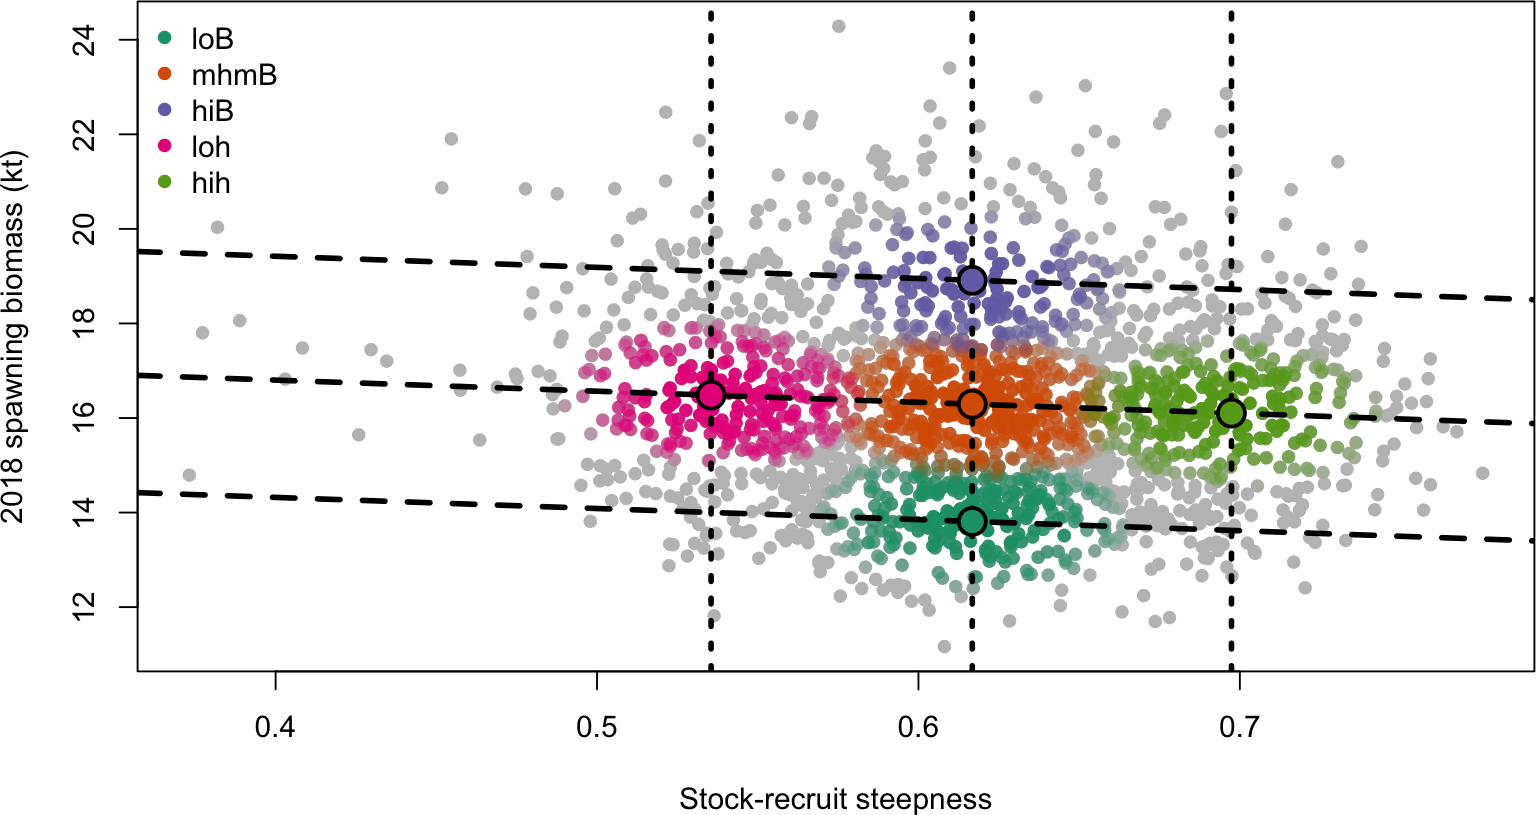
\includegraphics[width=0.9\linewidth]{knitr-figs-pdfunnamed-chunk-17-1}}{Figure \ref{fig:unnamed-chunk-17}} 

}

\caption{Échantillons par simulation MCCM de répartition conjointe et marginale a posteori (points gris) concernant l’inclinaison de la pente de la relation stock-recrutement ($h$; axe $x$) et la biomasse du stock reproducteur en 2018 ($B_{2018}$; axe $y$). Les lignes pointillées indiquent la médiane, les 10e et 90e centiles de chaque répartition marginale, alors que les centiles de la répartition de la biomasse du stock reproducteur sont rajustés pour correspondre à la droite de régression entre les deux répartitions marginales. Les points de couleur avec des bordures noires aux intersections de certains centiles sont les centres d’échantillonnage pour les cinq scénarios du modèle d’exploitation relatif à la productivité et à la biomasse, avec des étiquettes correspondant aux colonnes du tableau 1. Les échantillons par simulation MCCM a posteori en couleur montrent l’ensemble de tous les points à une distance de Mahalanobis de 0,6 du centre de la même couleur.}\label{fig:unnamed-chunk-17}
\end{figure}
\begin{figure}[htb]

{\centering \pdftooltip{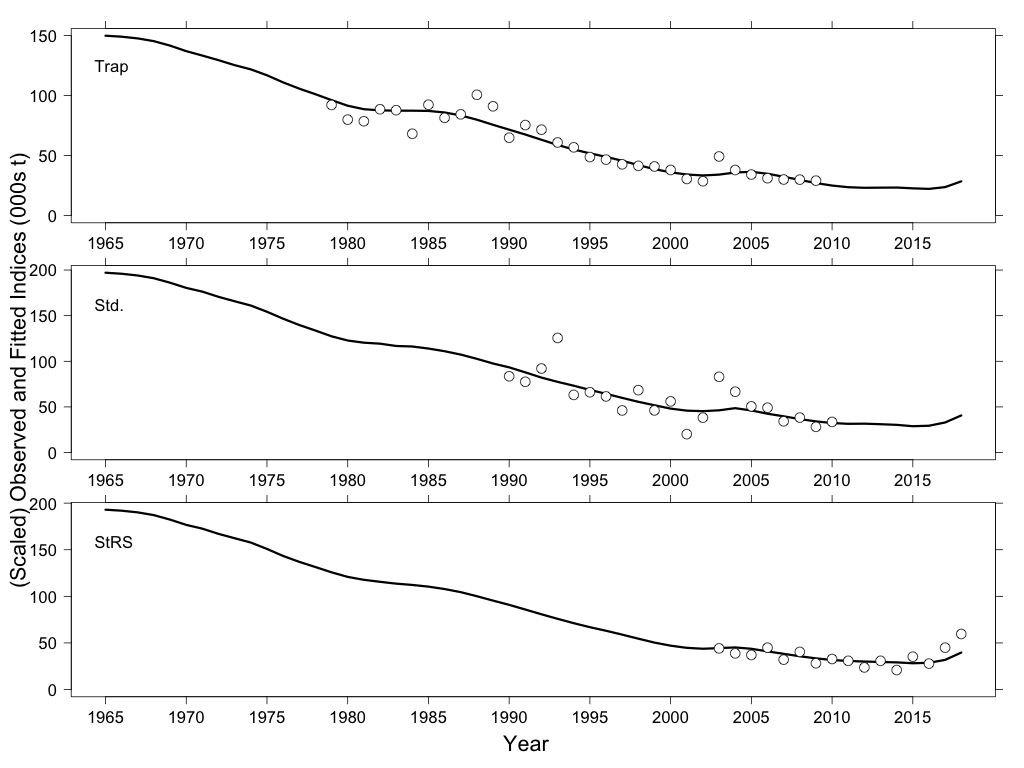
\includegraphics[width=0.9\linewidth]{data/base_ALK_mUnsexed/plotMLEindices}}{Figure \ref{fig:unnamed-chunk-19}} 

}

\caption{Ajustements du modèle d’exploitation par rapport aux indices de capture par unité d’effort (CPUE) [kg/casier] de la pêche commerciale au casier (Casier, haut), du relevé normalisé sur la morue charbonnière (Std, milieu) et du relevé aléatoire stratifié de la morue charbonnière (RASC, bas). Les points illustrent les observations dimensionnées selon la capturabilité, et les lignes montrent la biomasse vulnérable du modèle d’exploitation.}\label{fig:unnamed-chunk-19}
\end{figure}
\newpage
\begin{figure}[htb]

{\centering \pdftooltip{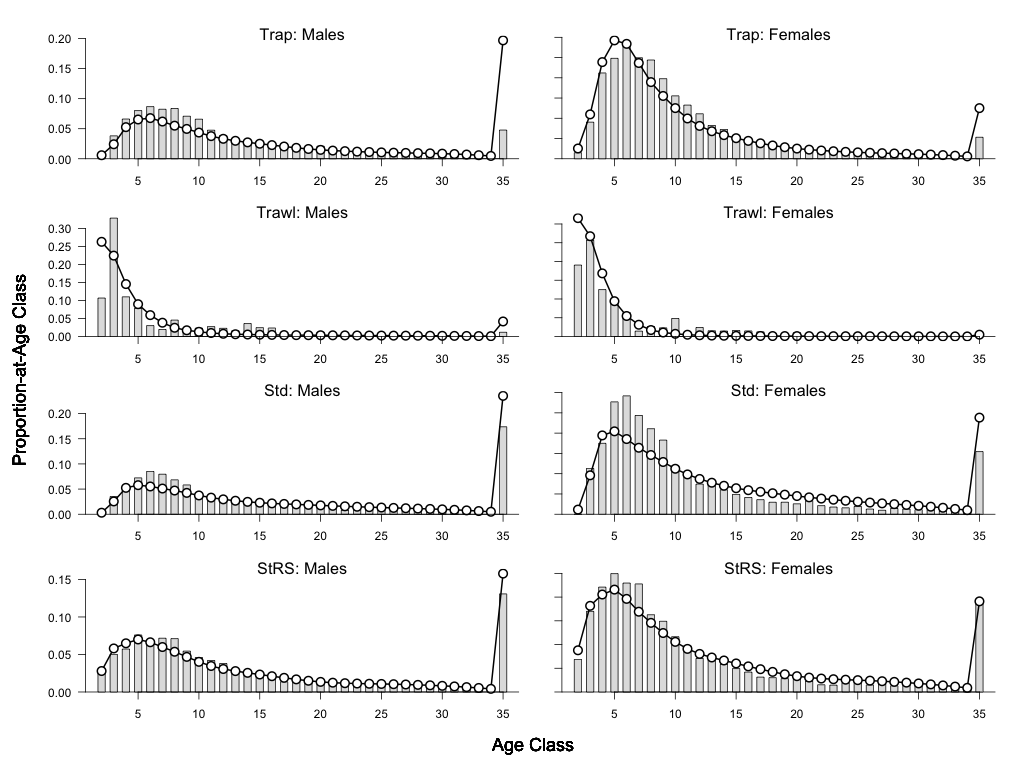
\includegraphics[width=0.9\linewidth]{data/base_ALK_mUnsexed/plotFitAgeFreq_avg}}{Figure \ref{fig:unnamed-chunk-20}} 

}

\caption{Modèle d’exploitation de la moyenne ajusté en fonction des observations sur l’âge, de haut en bas, pour la pêche commerciale au casier (Casier), la pêche commerciale au chalut (Chalut), le relevé normalisé (Std) et le relevé aléatoire stratifié (RASC). Les barres grises représentent la proportion moyenne des observations selon l’âge, et les points reliés par une ligne montrent la répartition moyenne prévue des observations selon l’âge dans le modèle d’exploitation. Les moyennes sont établies au fil des ans à partir d’observations.}\label{fig:unnamed-chunk-20}
\end{figure}
\newpage

\newpage
\begin{landscape}
\begin{figure}[htb]

{\centering \pdftooltip{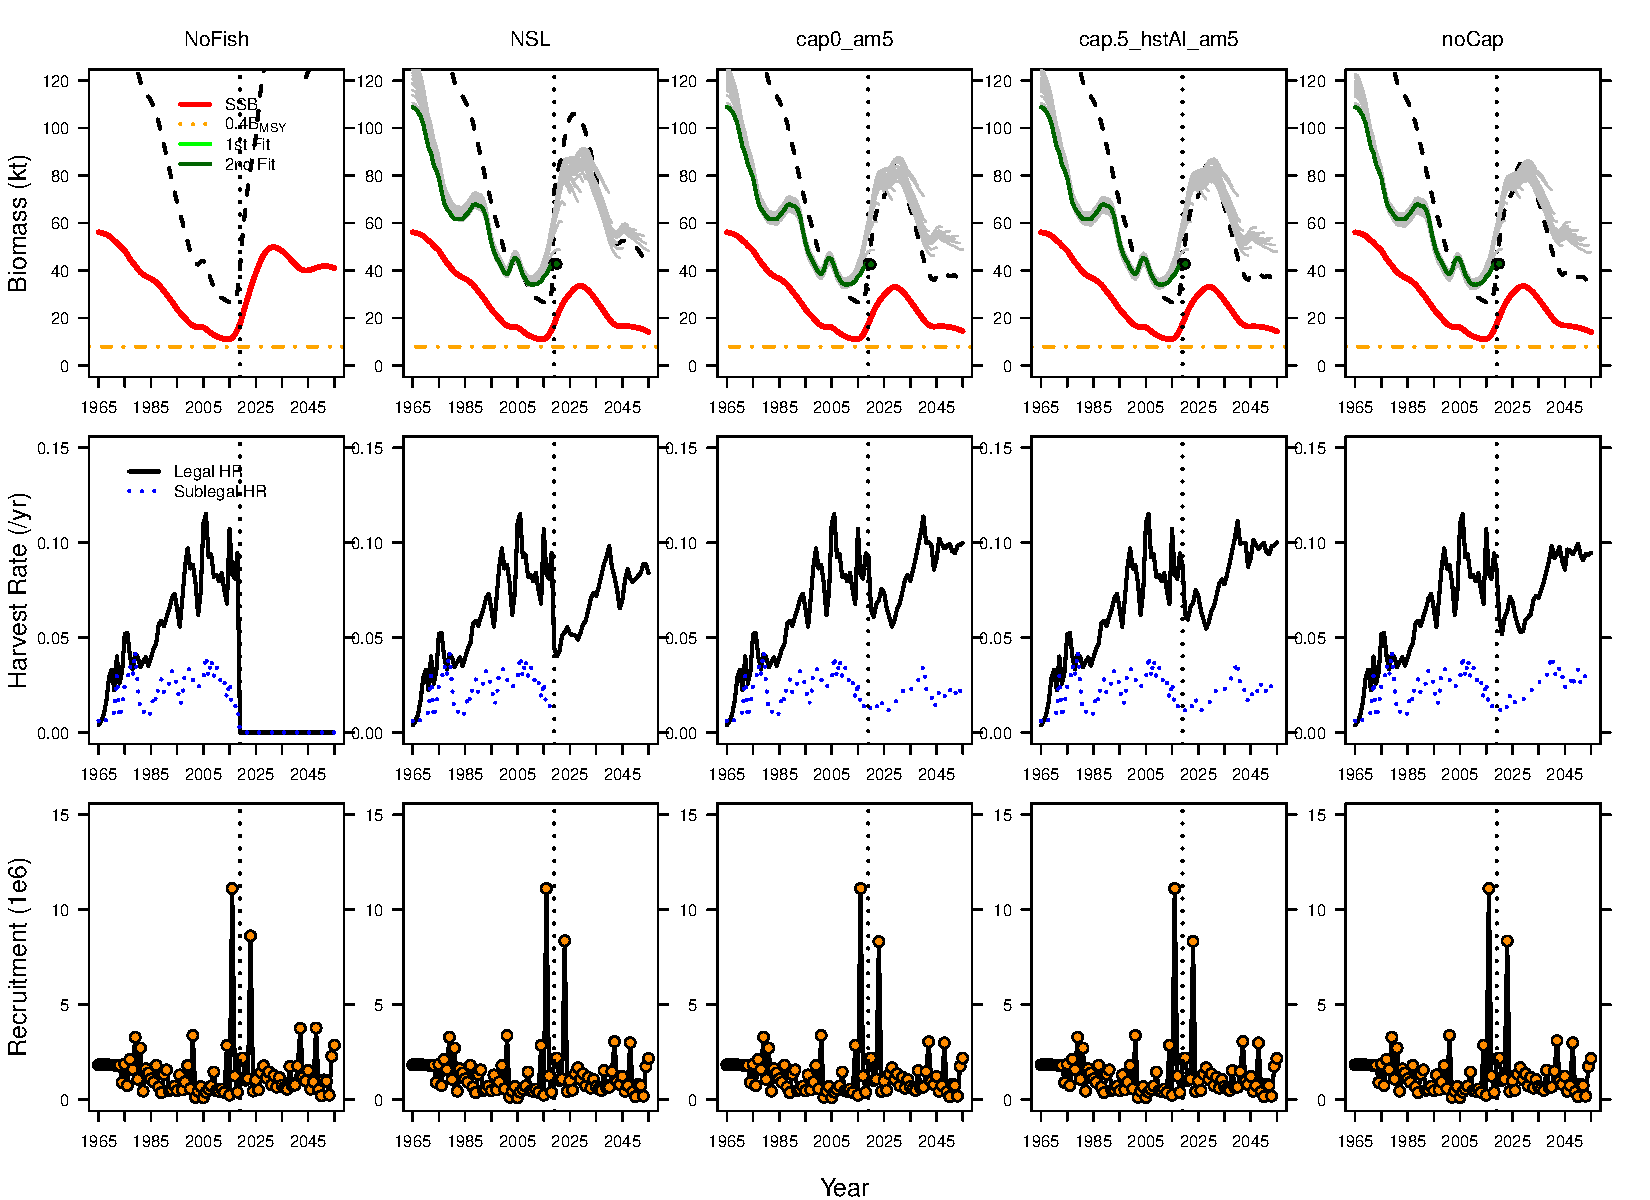
\includegraphics[width=0.9\linewidth]{data/BtFitUtRt/hiRec2016_wtd/hstAl_am5/BtFitUtRt_rep13}}{Figure \ref{fig:unnamed-chunk-22}} 

}

\caption{Reproduction unique d’une simulation tirée des \textbf{modèles d’exploitation de référence} avec une classe de 2015 à estimation élevée. La première rangée de panneaux montre la biomasse du stock reproducteur (ligne rouge), la biomasse légale (ligne pointillée noire) et la biomasse estimée du modèle de production excédentaire (lignes vertes et grises) lorsqu’elle est estimée dans le cadre de la procédure de gestion. La rangée du milieu illustre les taux de la récolte légale (ligne pleine noire) et de la récolte d’individus de taille inférieure (ligne pointillée bleue), tandis que la rangée du bas montre les recrutements selon le modèle d’exploitation (ligne noire avec points orange). Les premier et deuxième ajustements s’appliquent aux première et deuxième années d’application de la procédure de gestion.}\label{fig:unnamed-chunk-22}
\end{figure}
\newpage
\begin{figure}[htb]

{\centering \pdftooltip{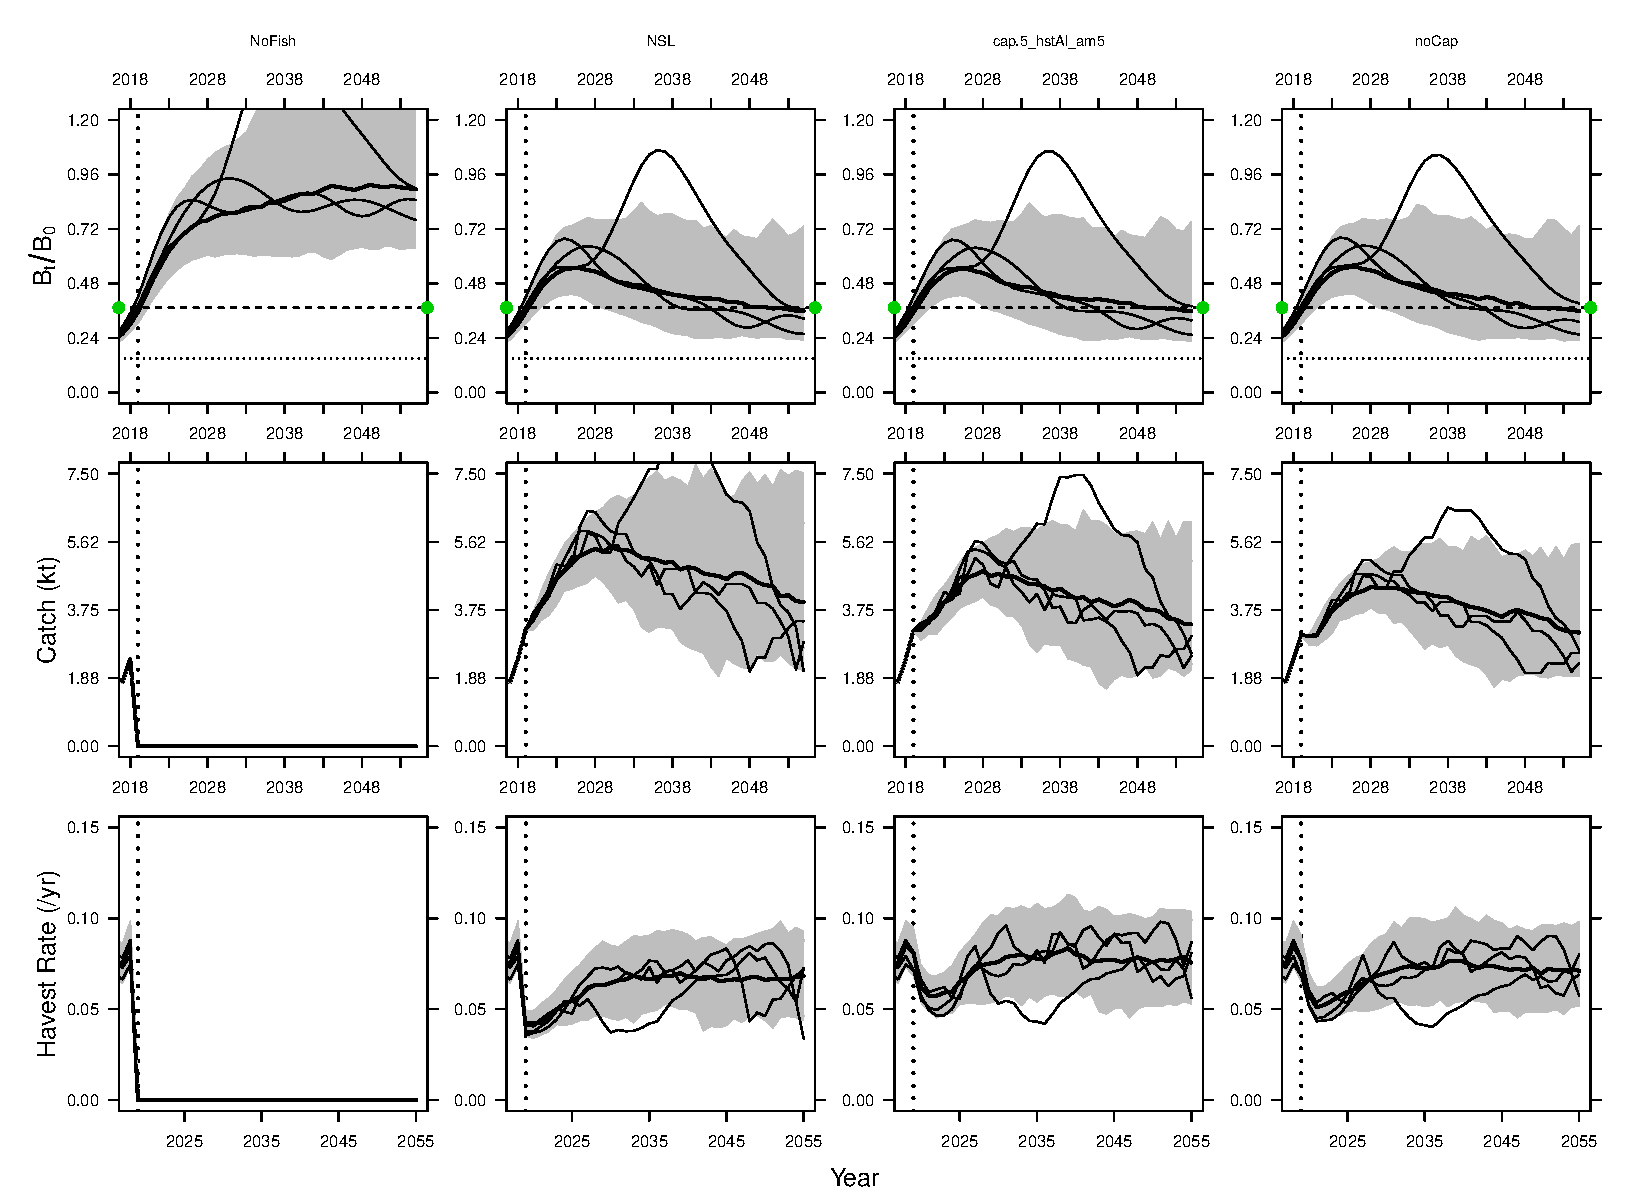
\includegraphics[width=0.9\linewidth]{data/tulipPlots/hiRec2016_wtd/depCatchHR/hiRec2016_wtd_depCatchHR_hstAl_am5}}{Figure \ref{fig:unnamed-chunk-24}} 

}

\caption{Enveloppes de simulation combinées et pondérées provenant des cinq modèles d’exploitation relatifs à la productivité et à la biomasse du \textbf{scénario de recrutement de référence} montrant la procédure de gestion actuelle (Aucun plafond), trois procédures de gestion illustrant la réglementation sur la remise à l’eau, et la procédure de gestion des stocks non exploités (Population non exploitée). La rangée du haut montre la biomasse projetée par rapport à la population non exploitée, la deuxième rangée illustre les prises débarquées, et celle du bas fournit le taux de récolte légale. Dans chaque panneau, les projections médianes sont représentées par des lignes noires épaisses, le centile central (90 \%) de l’enveloppe est ombré en gris, et les trois reproductions des simulations illustrées correspondent à de minces lignes noires.}\label{fig:unnamed-chunk-24}
\end{figure}
\newpage
\begin{figure}[htb]

{\centering \pdftooltip{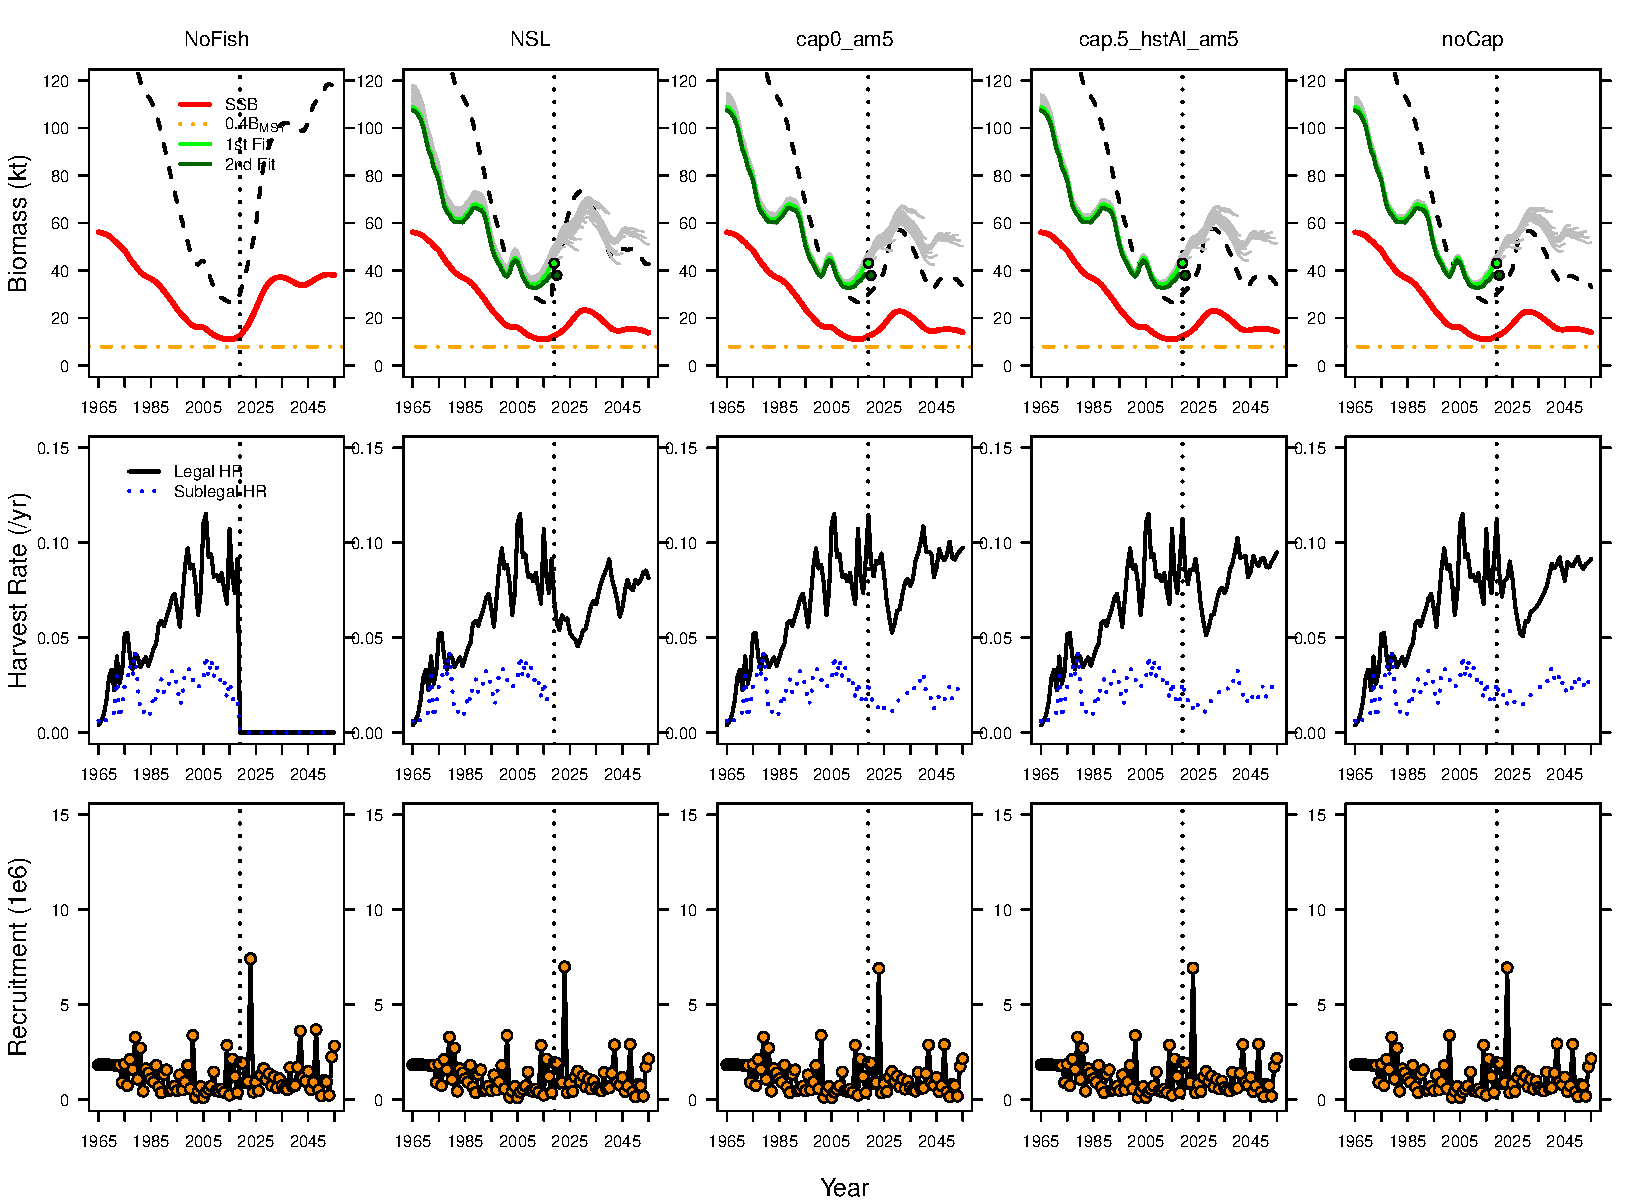
\includegraphics[width=0.9\linewidth]{data/BtFitUtRt/simRec2016_wtd/hstAl_am5/BtFitUtRt_rep13}}{Figure \ref{fig:unnamed-chunk-25}} 

}

\caption{Reproduction unique d’une simulation tirée des \textbf{modèles d’exploitation de robustesse} avec une classe de 2015 simulée de manière stochastique. La première rangée de panneaux montre la biomasse du stock reproducteur (ligne rouge), la biomasse légale (ligne pointillée noire) et la biomasse estimée du modèle de production excédentaire (lignes vertes et grises) lorsqu’elle est estimée dans le cadre de la procédure de gestion. La rangée du milieu illustre les taux de la récolte légale (ligne pleine noire) et de la récolte d’individus de taille inférieure (ligne pointillée bleue), tandis que la rangée du bas montre les recrutements selon le modèle d’exploitation (ligne noire avec points orange). Les premier et deuxième ajustements s’appliquent aux première et deuxième années d’application de la procédure de gestion.}\label{fig:unnamed-chunk-25}
\end{figure}
\newpage
\begin{figure}[htb]

{\centering \pdftooltip{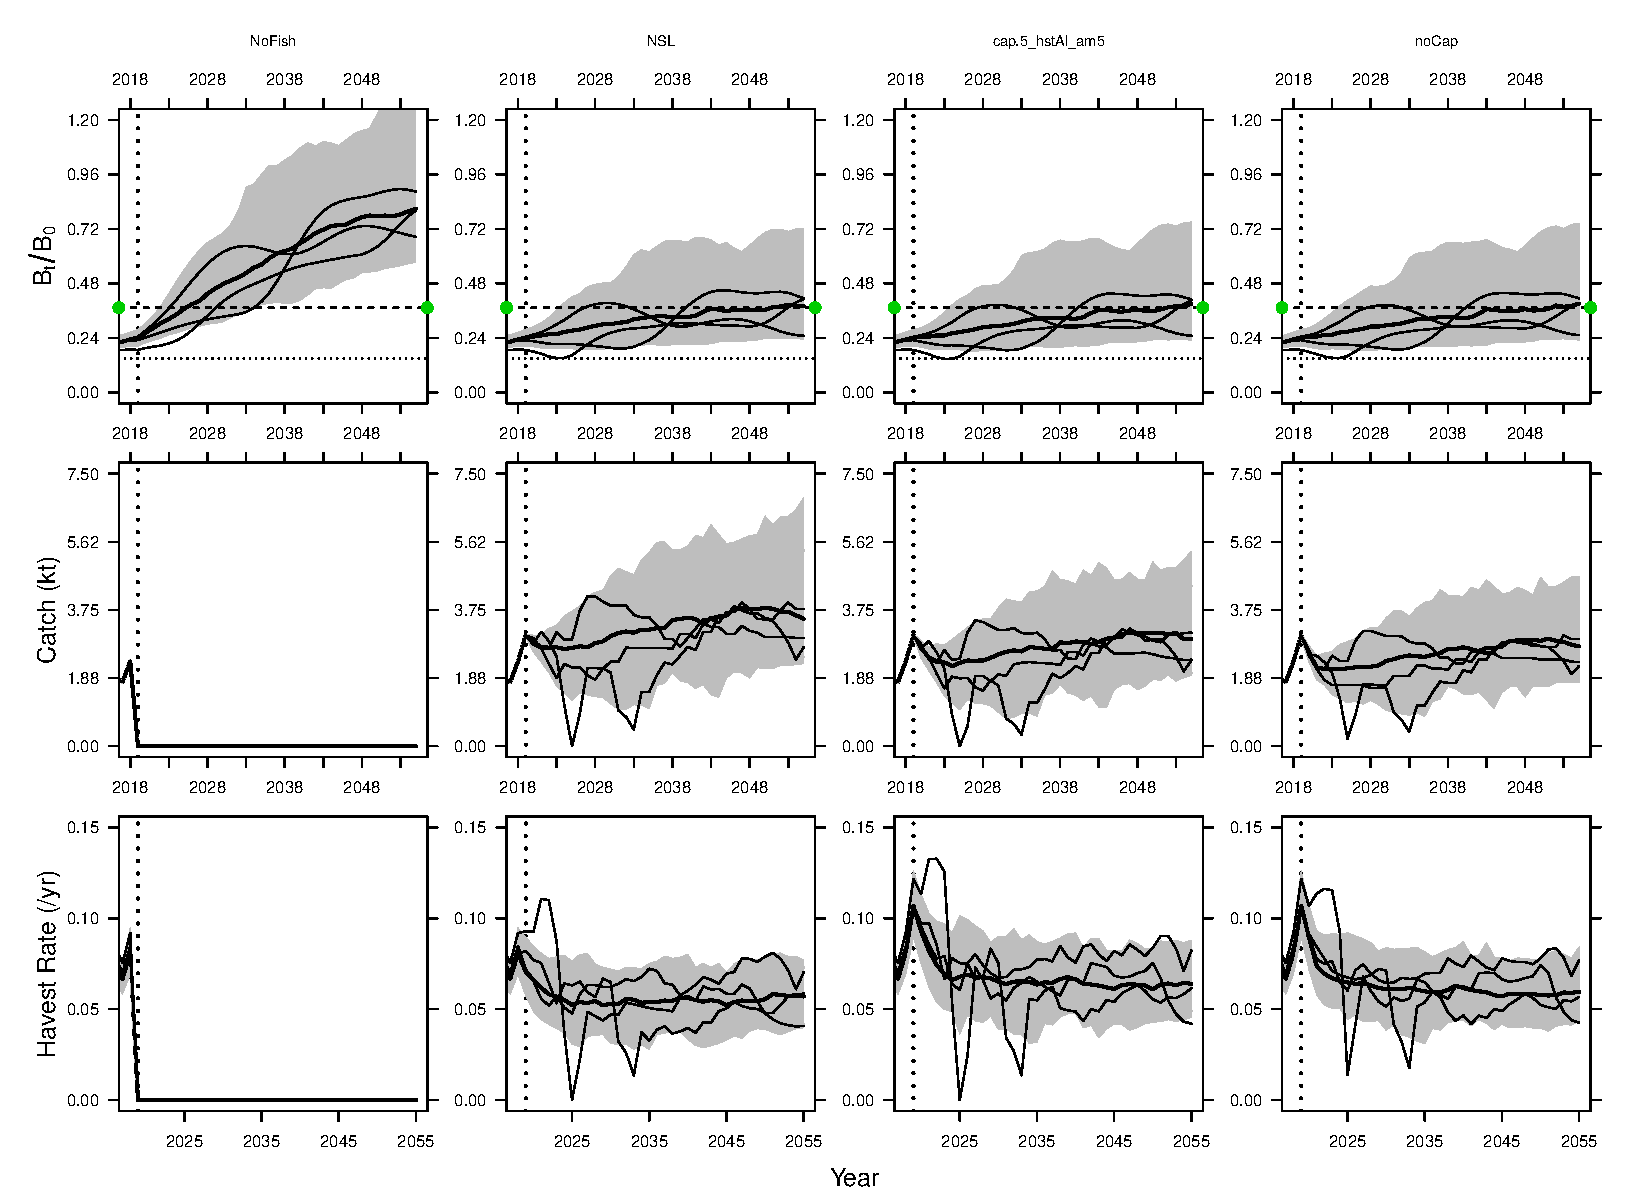
\includegraphics[width=0.9\linewidth]{data/tulipPlots/simRec2016_wtd/depCatchHR/simRec2016_wtd_depCatchHR_hstAl_am5}}{Figure \ref{fig:unnamed-chunk-26}} 

}

\caption{Enveloppes de simulation combinées et pondérées provenant des cinq modèles d’exploitation relatifs à la productivité et à la biomasse du \textbf{scénario de recrutement de robustesse} montrant la procédure de gestion actuelle (Aucun plafond), trois procédures de gestion illustrant la réglementation sur la remise à l’eau, et la procédure de gestion des stocks non exploités (Population non exploitée). La rangée du haut montre la biomasse projetée par rapport à la population non exploitée, la deuxième rangée illustre les prises débarquées, et celle du bas fournit le taux de récolte légale. Dans chaque panneau, les projections médianes sont représentées par des lignes noires épaisses, le centile central (90 \%) de l’enveloppe est ombré en gris, et les trois reproductions des simulations illustrées correspondent à de minces lignes noires.}\label{fig:unnamed-chunk-26}
\end{figure}
\end{landscape}
\hypertarget{annexe}{%
\section{\texorpdfstring{Annexe \label{sec:app-minor}}{Annexe }}\label{annexe}}

\hypertarget{mise-uxe0-jour-de-la-matrice-des-erreurs-de-duxe9termination-de-luxe2ge}{%
\subsection{Mise à jour de la matrice des erreurs de détermination de l'âge}\label{mise-uxe0-jour-de-la-matrice-des-erreurs-de-duxe9termination-de-luxe2ge}}

Le modèle d'évaluation fondé sur l'âge de la morue charbonnière utilise les données relatives aux prises selon l'âge pour estimer la véritable composition de la population en fonction de l'âge; toutefois, les données observées à ce titre proviennent de lectures d'otolithes qui sont mal connues. Le fait de ne pas tenir compte des erreurs dans les lectures d'otolithes peut entraîner des estimations lissées des classes d'âge et ainsi rendre plus difficile la détection des grandes années de recrutement ou des relations stock-recrutement (Hanselman et al. \protect\hyperlink{ref-hanselman2012statistical}{2012}). Les erreurs de détermination de l'âge peuvent également fausser les estimations des paramètres de croissance, les calendriers de maturation et les taux de mortalité naturelle et mener en conséquence à la surpêche ou à des projections inexactes du rendement (Lai and Gunderson \protect\hyperlink{ref-lai1987effects}{1987}; Tyler et al. \protect\hyperlink{ref-tyler1989implications}{1989}).

Pour tenir compte des erreurs liées à l'âge, le modèle d'exploitation structuré selon l'âge de la morue charbonnière utilise une matrice des erreurs de détermination de l'âge. Aux fins du présent cycle d'évaluation des stratégies de gestion, nous avons simplifié la formule de la matrice des erreurs de détermination de l'âge en remplaçant le modèle à double géométrie appliqué précédemment par une répartition discrétisée normale. Les deux principales différences entre ces deux formules sont les suivantes : i) la structure d'erreur est limitée de manière à assurer la symétrie avec la formule normale, tandis que le modèle à double géométrie permet une certaine asymétrie dans la répartition des erreurs; et ii) la formule normale tient pour acquis que l'âge réel assigné est le mode de la densité normale, de sorte que les erreurs d'âge ne sont en moyenne pas biaisées.

Pour constituer notre matrice d'erreurs de détermination de l'âge, nous avons utilisé des otolithes qui avaient été lus par deux lecteurs différents au laboratoire de scalimétrie de la Station biologique du Pacifique du MPO. Ces données représentent environ 15~\% des lectures d'otolithes totales pour la morue charbonnière de la Colombie-Britannique; elles sont lues d'abord par le lecteur principal, puis par un lecteur secondaire qui assure le contrôle de la qualité. Dans la majorité des cas, les lecteurs étaient d'accord (62~\%). Dans les cas où ils différaient d'opinion (38~\%), ils se sont consultés pour résoudre l'écart et se sont entendus sur l'âge final attribué (comm. pers., J. Groot, MPO). Dans la plupart des cas, la lecture finale selon l'âge était celle attribuée par le lecteur secondaire ou primaire (36~\%), mais dans quelques cas, un nouvel âge a été retenu (2~\%).

Nous avons appliqué des modèles statistiques pour estimer la probabilité d'observation d'une classe d'âge a) compte tenu de l'âge réel b) selon les méthodes décrites dans Richards et al. (\protect\hyperlink{ref-richards1992statistical}{1992}) et Heifetz et al. (\protect\hyperlink{ref-heifetz1999age}{1999}). Le modèle suppose une répartition normale des erreurs de détermination de l'âge où l'écart-type estimé de l'âge observé pour un véritable âge b est fondé sur trois paramètres \(\Phi = \{ \sigma_1, \sigma_A, \alpha \}\) de la manière suivante :
\begin{equation}
\sigma(b) = \left\{
 \begin{array}{ll}
  \sigma_1 + (\sigma_A – \sigma_1) \frac{1 – e^{-\alpha(b – 1)} }{1 – e^{-\alpha(A – 1)}}, & \alpha \neq 0; \\
  \sigma_1 + (\sigma_A – \sigma_1) \frac{b-1}{A-1}, & \alpha = 0.\\
 \end{array} \right.
\end{equation}
Les paramètres \(\sigma_1\) et \(\sigma_A\) sont les écarts-types pour \(b=1\) et \(b=A\), qui représentent respectivement les âges minimal et maximal. Le paramètre \(\alpha\) détermine la non-linéarité de la fonction, de sorte que \(\sigma(b)\) devient linéaire comme \(\alpha \rightarrow 0\). La matrice des erreurs de détermination de l'âge est définie comme suit :
\begin{align}
q(a ~|~ b, \Phi) &= \frac{x_{ab}(\Phi)}{\sum_{a = 1}^A x_{ab}(\Phi) }; \\x_{ab} &= \frac{1}{\sqrt{2\pi}\sigma(b)} e^{-\frac12 \left[ \frac{a-b}{\sigma(b)} \right]^2}.
\end{align}
Étant donné que l'âge réel des poissons est inconnu, il est impossible de déterminer avec précision le biais dans les lectures d'âge et d'établir si certaines classes d'âge sont plus susceptibles d'être sous-estimées ou surestimées. Nous avons essayé deux approches différentes pour déterminer l'« âge réel » présumé, soit 1) la moyenne des âges attribuées par les deux lecteurs arrondie au nombre entier le plus proche (Heifetz et al. \protect\hyperlink{ref-heifetz1999age}{1999}), et 2) l'âge final attribué. Pour les deux approches, nous établissons \(A=90\) en fonction de l'âge maximal attribué par les lecteurs.

La probabilité \(\mathcal{L}\) des âges \(A\) observés compte tenu des âges réels B est alors définie comme suit :
\begin{equation}
\mathcal{L}(A|B) = \prod_{i = 1}^I \prod_{j = 1}^J q(a_{ij} ~|~ b_i \Phi),\end{equation}

où \(b_i\) est l'« âge réel » présumé du poisson \(i\), et \(a_{ij}\) est l'âge attribué par le lecteur \(j\) au poisson individuel \(i\). Les estimations maximales des paramètres de probabilité, l'écart-type prévu à l'âge et les matrices d'erreurs de détermination de l'âge sont fournies ci-dessous (tableau A1, figures A1 et A2).

\hypertarget{cluxe9-uxe2ge-longueur-pour-chalut-et-courbe-de-suxe9lectivituxe9-mise-uxe0-jour}{%
\subsection{Clé âge-longueur pour chalut et courbe de sélectivité mise à jour}\label{cluxe9-uxe2ge-longueur-pour-chalut-et-courbe-de-suxe9lectivituxe9-mise-uxe0-jour}}

Le modèle d'exploitation structuré en fonction de l'âge de la morue charbonnière utilise des observations sur des prises selon l'âge provenant de la pêche commerciale pour estimer les fonctions de mortalité naturelle et de sélectivité des engins. La sélectivité des chaluts constitue un déterminant clé de la diminution des estimations inexactes relatives aux prises et remises à l'eau de morues charbonnières de taille inférieure à la taille réglementaire (Cox et al. \protect\hyperlink{ref-cox2019evaluating}{2019}). Jusqu'à maintenant, le modèle de sélectivité des chaluts dépendait fortement des valeurs antérieures pour une courbe de sélectivité estimée à partir du rétablissement de poissons étiquetés (dans l'année suivant leur remise à l'eau) dans le cadre de la pêche commerciale par chalut. Pour améliorer les estimations de la mortalité des poissons de taille réglementaire et de ceux de taille inférieure à la taille réglementaire dans le secteur du chalutage, nous avons utilisé les données sur les prises selon l'âge et les prises selon la longueur provenant du secteur du chalutage en Colombie-Britannique pour établir une clé âge longueur selon le sexe, qui a ensuite servi à élargir la taille de l'échantillon de prises selon l'âge.

Pour définir notre clé âge-longueur, nous avons utilisé toutes les données disponibles sur les prises selon l'âge recueillies lors des sorties observées dans le cadre de la pêche commerciale au chalut. Ces données ont ensuite servi à alimenter la matrice empirique des fréquences selon l'âge, en plaçant les poissons dans des casiers de 3 cm de longueur et dans des classes d'âge d'un an. Nous avons établi cette matrice comme suit : \begin{equation}
F = \left[ n_{l,a} \right],
\end{equation} où \(n_{l,a}\) est le nombre de poissons observés dans le casier de longueur \(l\) et la classe d'âge \(a\). La matrice \(A\) a été convertie en une matrice de probabilité \(P\) selon l'âge et la longueur \(l\) \$ au moyen de la normalisation des colonnes de \(A\). \begin{equation}
P_{l,a} = F_{l,a} / \sum_{a'} F_{l,a'}
\end{equation}
Nous avons ensuite produit des données sur la composition en fonction de l'âge prévue en appliquant la matrice \(P\) aux compositions selon la longueur \(C_l\) dérivées des données sur les prises selon la longueur du chalutage commercial. \begin{align}
C_a &= P^T \cdot C_l,
\end{align} où \(P\) est transposé de façon à ce que la dimension relative à la longueur corresponde au vecteur \(C_l\). Nous avons inclus dans \(C_l\) seulement les données sur les prises selon la longueur des années où au moins cinq sorties ont été échantillonnées. Nous avons défini les clés \(P_m\) et \(P_f\) pour les poissons mâles et femelles, respectivement, et généré des observations selon l'âge pour chaque sexe (figures A3 et A4). Aux fins des observations sur la longueur, les poissons de sexe indéterminé ont été traités comme des spécimens mâles, puisque l'optimisation du modèle d'exploitation ne convergerait pas s'ils étaient considérés comme des poissons femelles.
Les compositions déduites des prises selon l'âge ont eu un effet notable sur les courbes de sélectivité en fonction de la longueur pour la flottille de chalutage (figure A5). La classe de taille avec une pleine sélectivité est passée d'environ 42 cm à 48 cm, et la forme du dôme de la courbe de sélection Gamma était plus étroite, ce qui a entraîné une désélection d'environ 60 \% des poissons en raison de la limite de taille de 55 cm, comparativement à environ 80 \% pour le modèle normal en 2016.

\newpage
\begin{longtable}[]{@{}rlrrr@{}}
\caption{\label{tab:unnamed-chunk-28}Paramètres du modèle d'erreur de détermination de l'âge pour les deux cas d'âge réel testés.}\tabularnewline
\toprule
Cas & Âge réel & \(\sigma_1\) & \(\sigma_A\) & \(\alpha\)\tabularnewline
\midrule
\endfirsthead
\toprule
Cas & Âge réel & \(\sigma_1\) & \(\sigma_A\) & \(\alpha\)\tabularnewline
\midrule
\endhead
1 & Âge moyen attribué par les lecteurs & 0.38 & 4.80 & 0.014\tabularnewline
2 & Âge final attribué & 0.89 & 9.35 & -0.008\tabularnewline
\bottomrule
\end{longtable}
\newpage
\begin{figure}[htb]

{\centering \pdftooltip{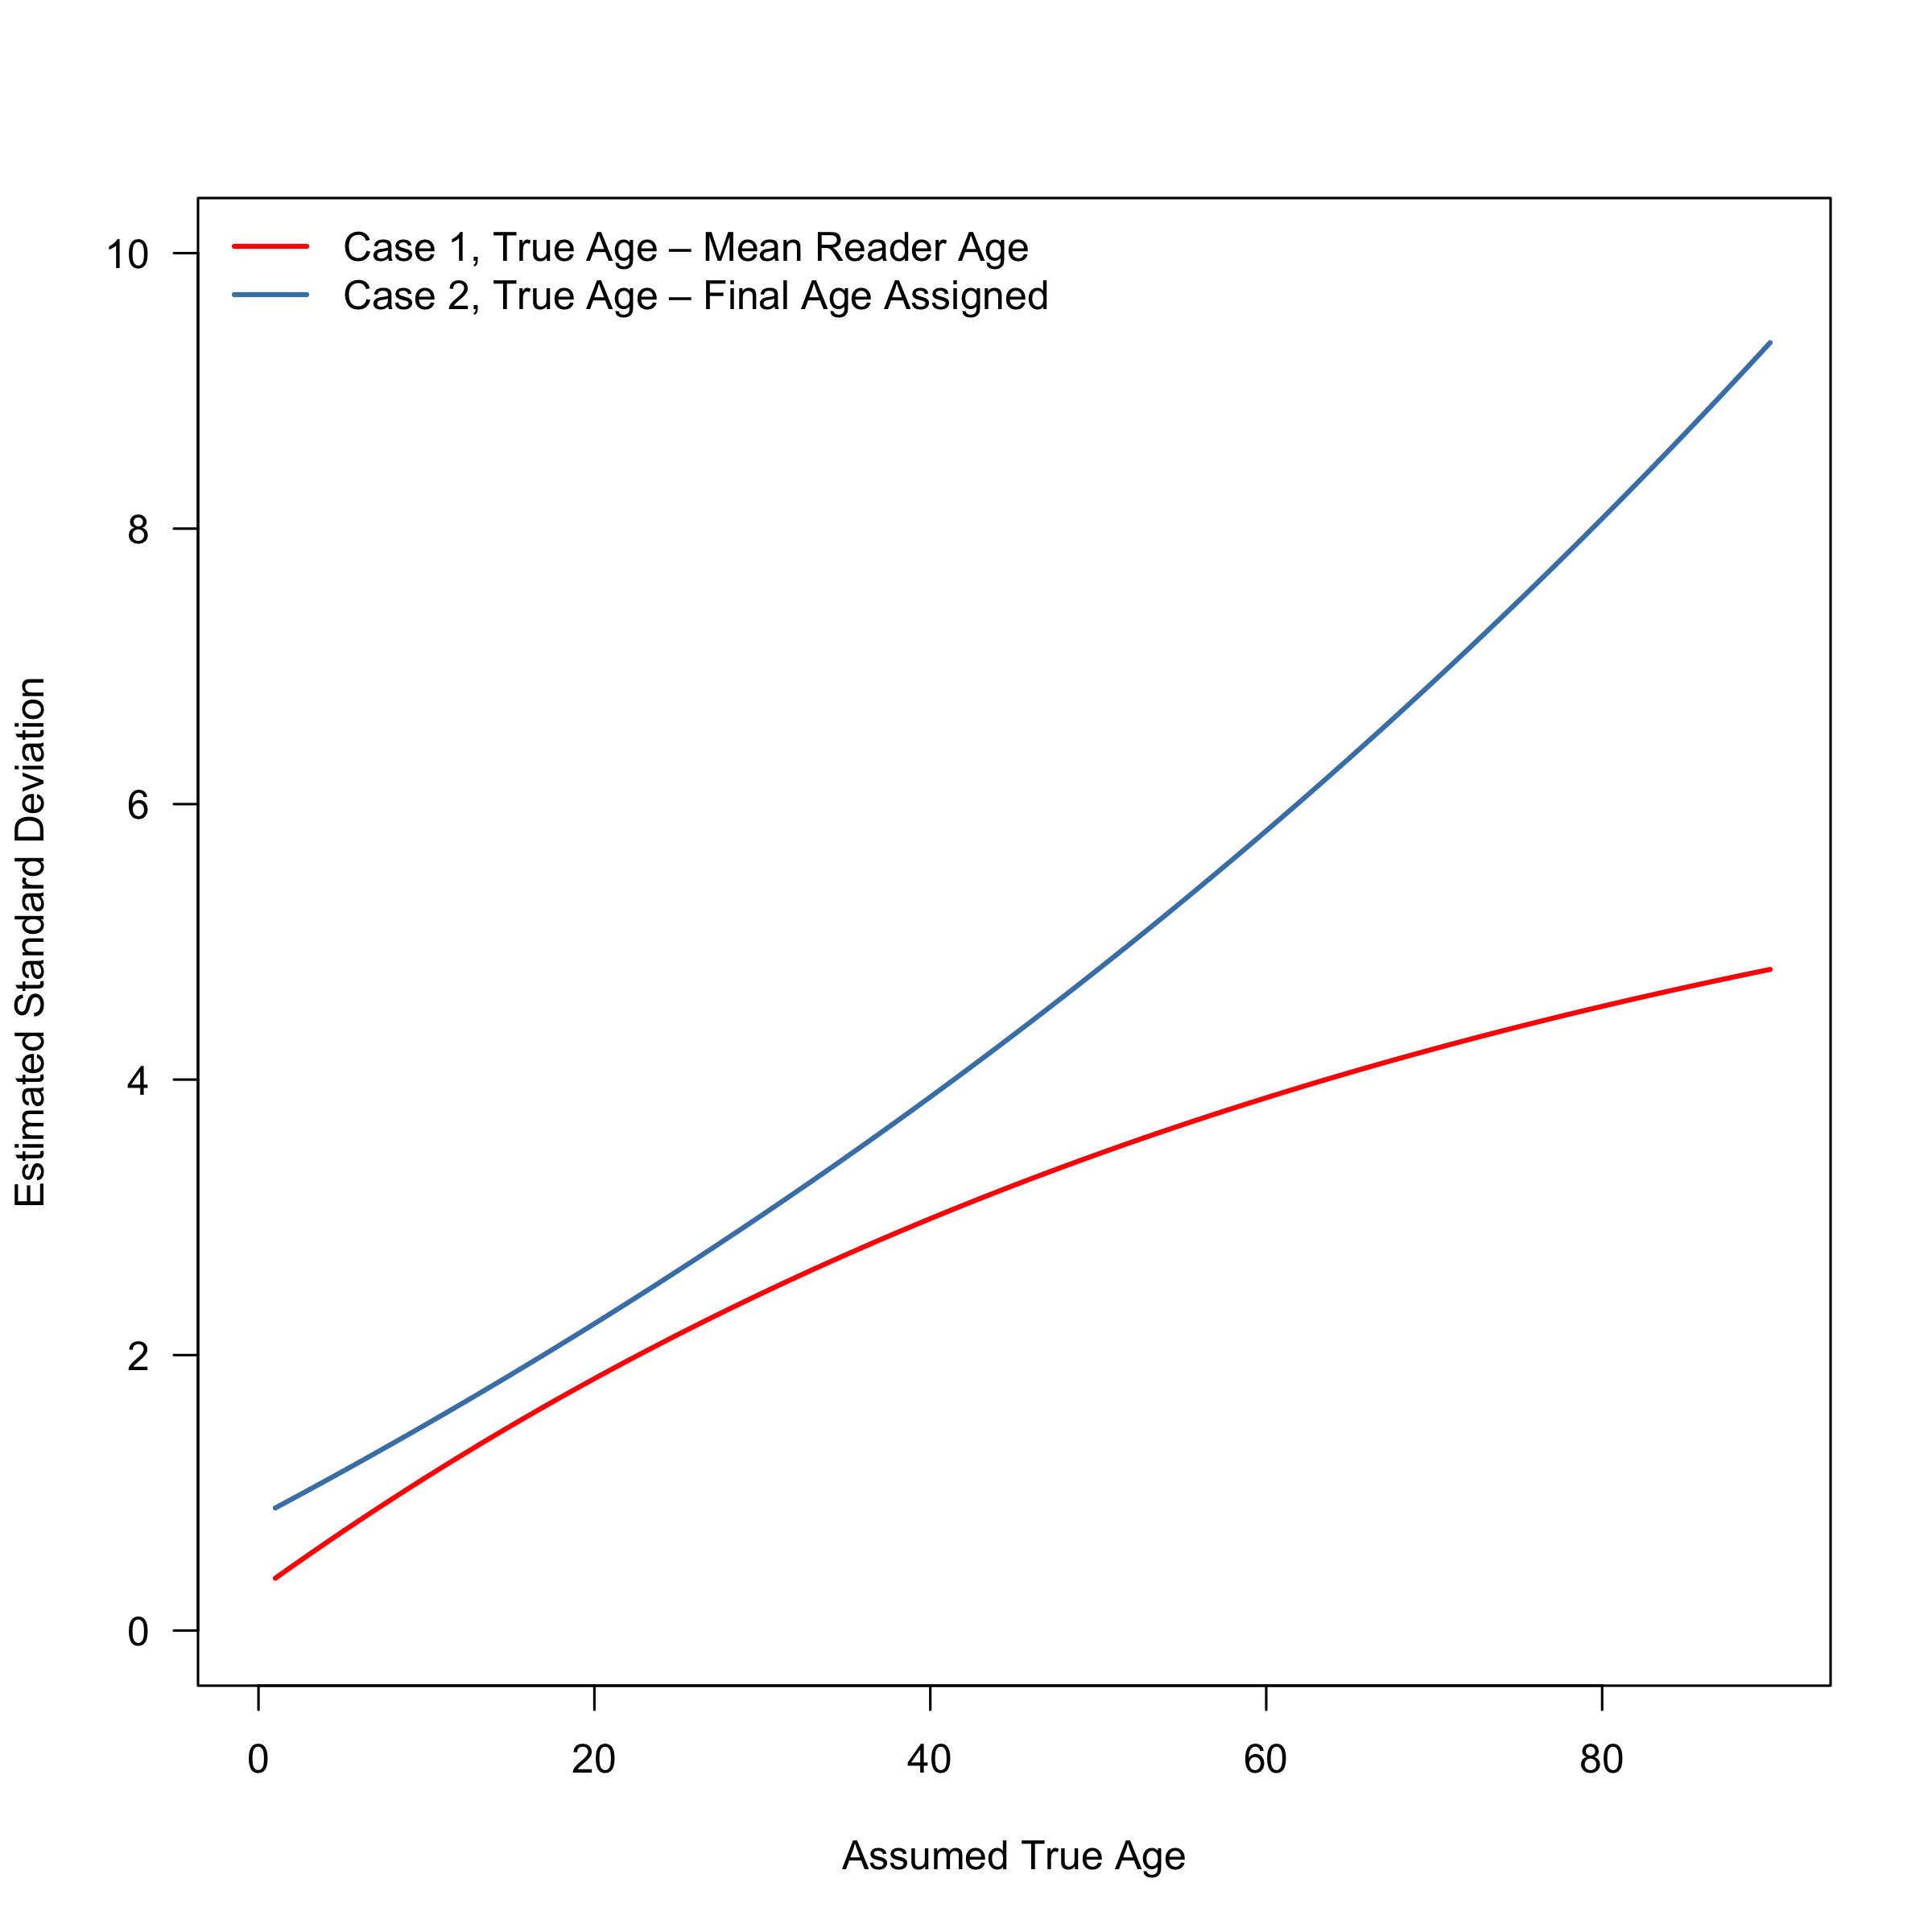
\includegraphics[width=0.9\linewidth]{data/ageErr1}}{Figure \ref{fig:unnamed-chunk-30}} 

}

\caption{Estimation de l’écart-type des âges observés pour les deux cas d’attribution de l’âge examinés.}\label{fig:unnamed-chunk-30}
\end{figure}
\newpage
\begin{figure}[htb]

{\centering \pdftooltip{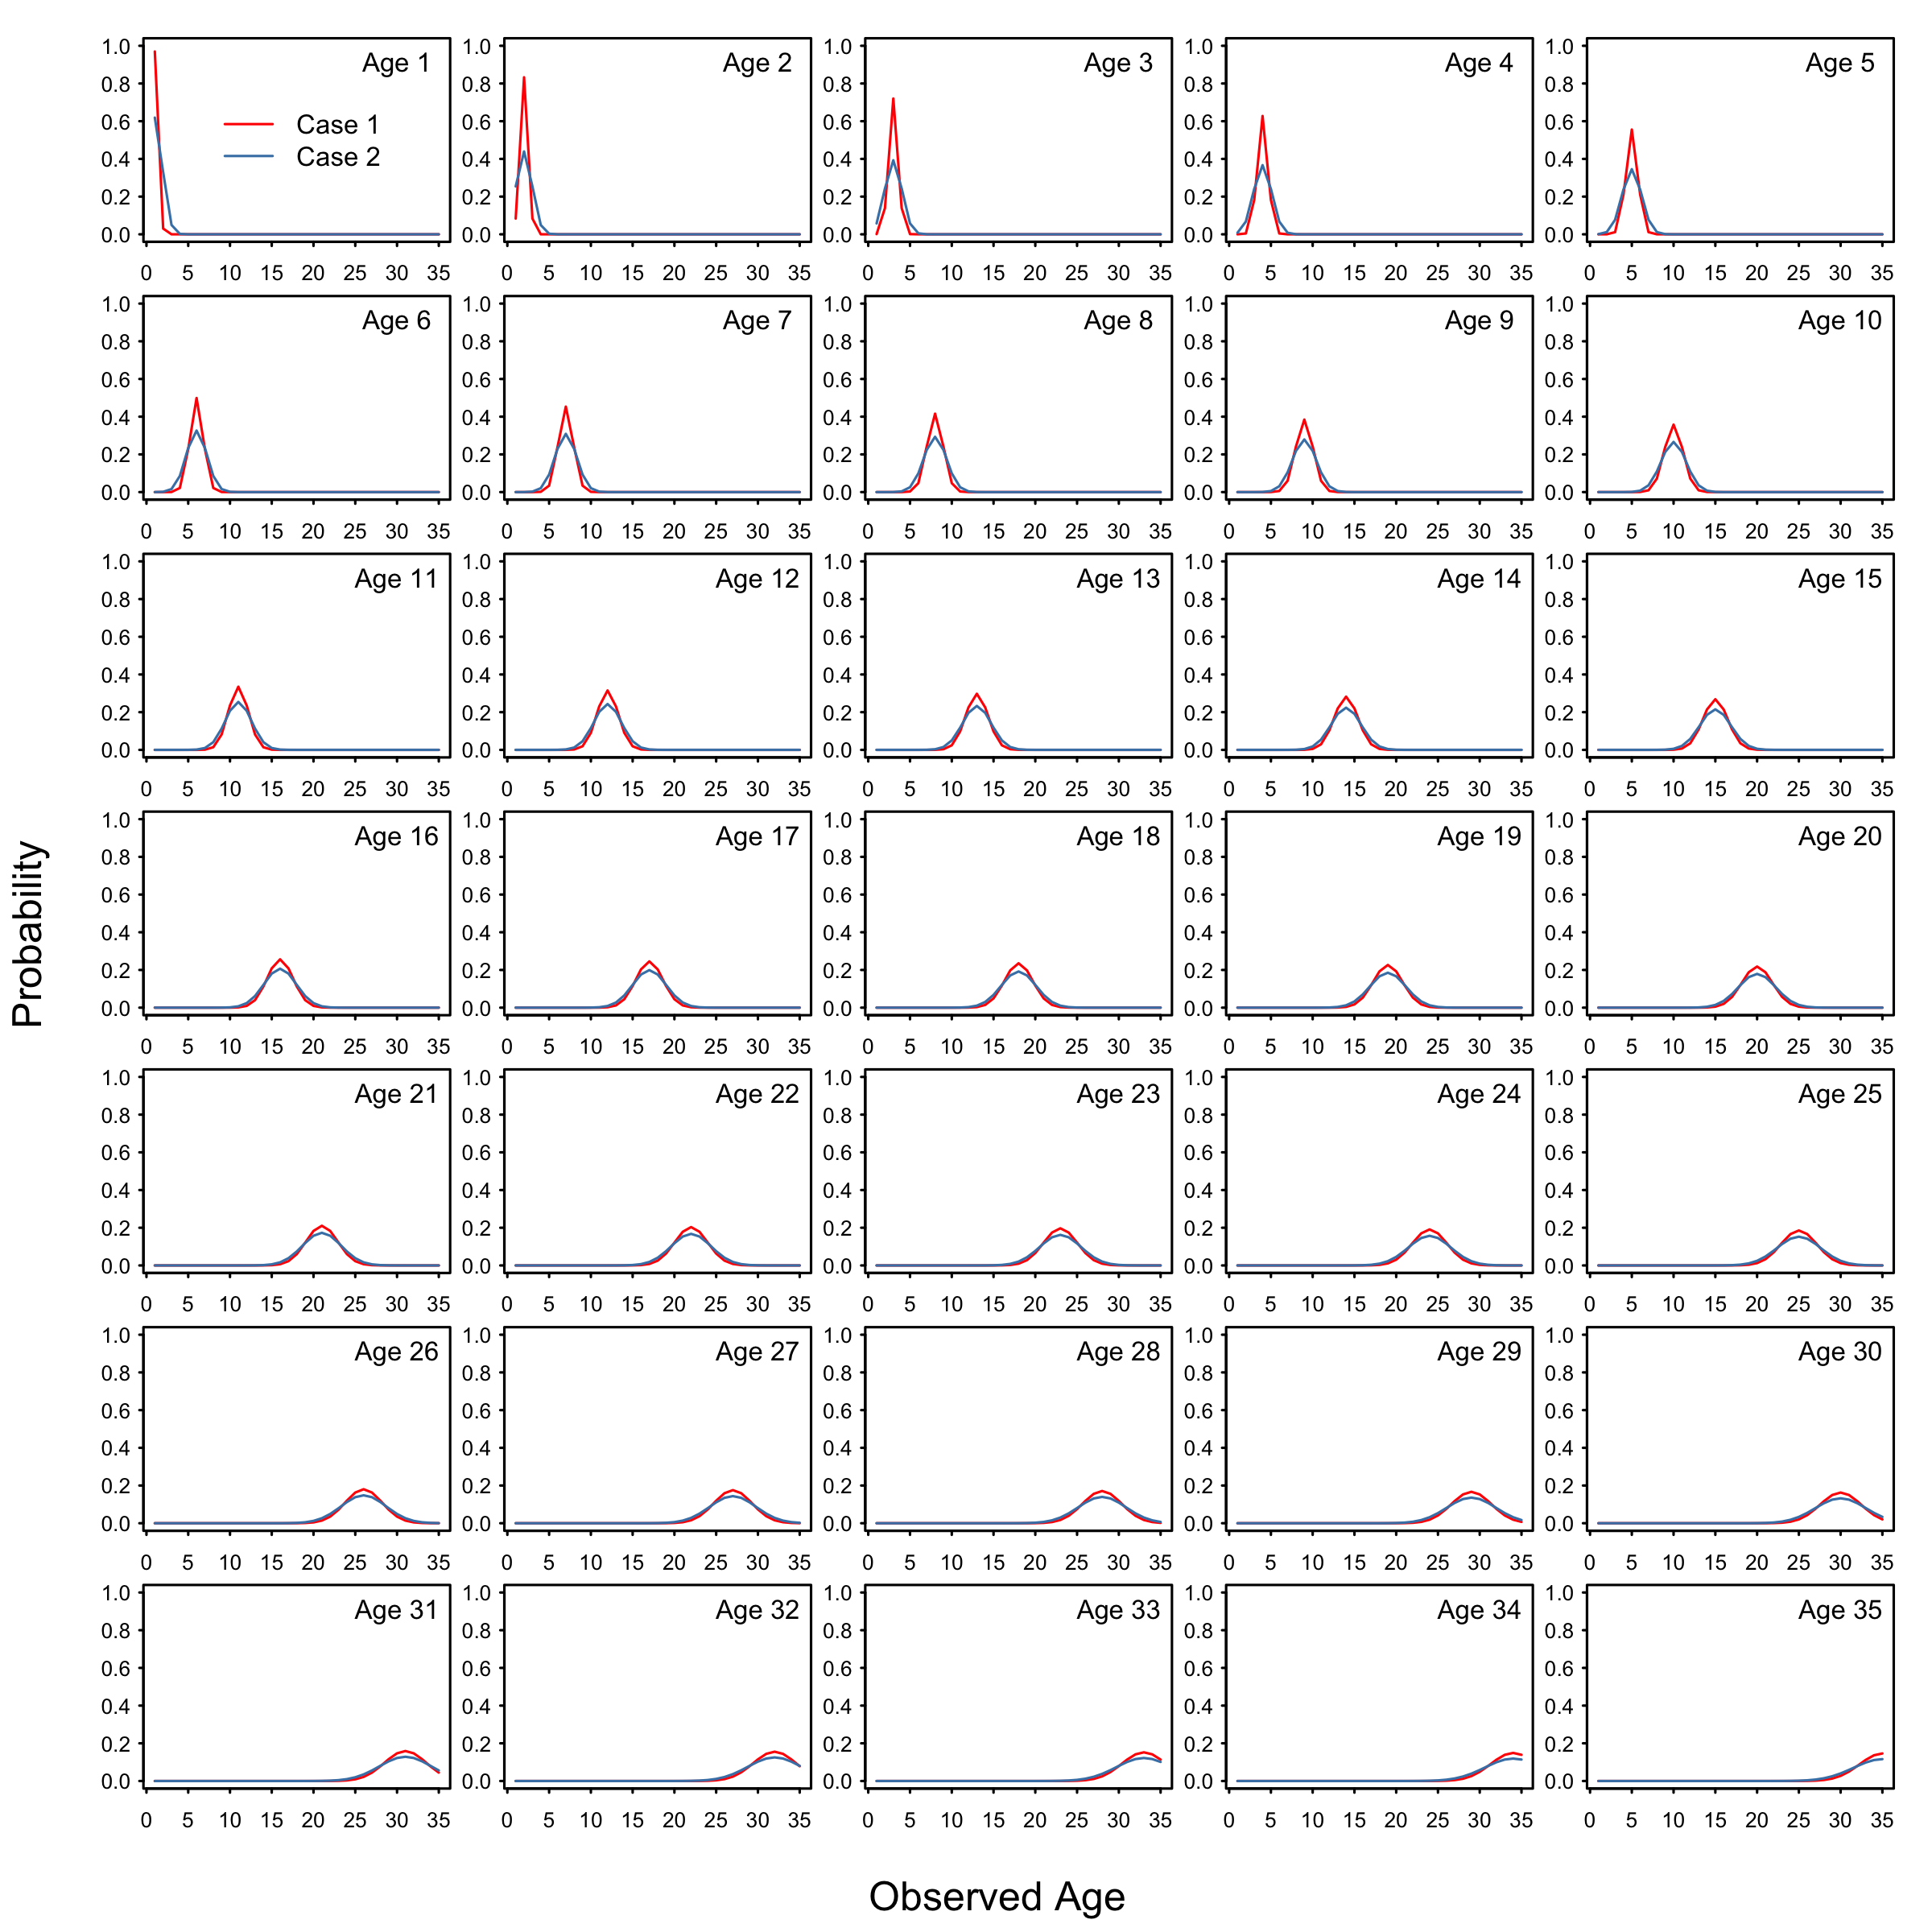
\includegraphics[width=0.9\linewidth]{data/ageErr2}}{Figure \ref{fig:unnamed-chunk-31}} 

}

\caption{Probabilité des âges observés compte tenu de l’âge réel indiqué dans le coin supérieur droit de chaque panneau pour les deux cas d’attribution de l’âge examinés}\label{fig:unnamed-chunk-31}
\end{figure}
\newpage
\begin{figure}[htb]

{\centering \pdftooltip{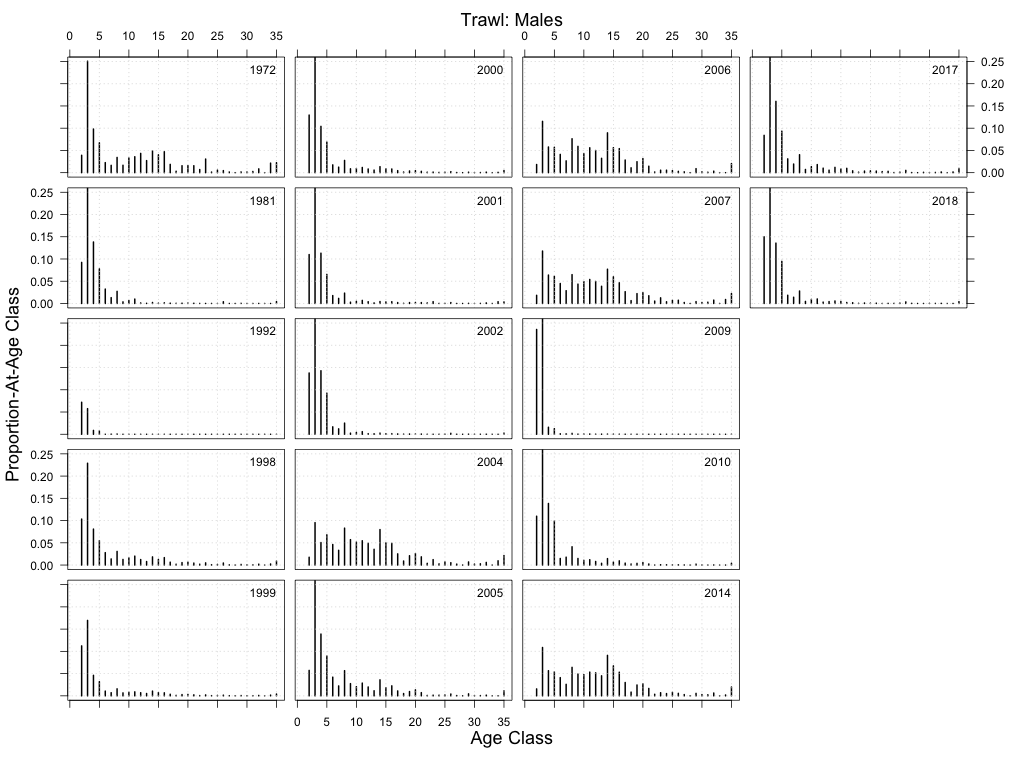
\includegraphics[width=0.9\linewidth]{data/base_ALK_mUnsexed/plotObsAgeFreq_m3}}{Figure \ref{fig:unnamed-chunk-32}} 

}

\caption{Compositions estimées des prises mâles selon l’âge qu’a générées la clé âge longueur de la pêche au chalut créée à partir des observations sur la longueur des poissons mâles et de sexe indéterminé.}\label{fig:unnamed-chunk-32}
\end{figure}
\newpage
\begin{figure}[htb]

{\centering \pdftooltip{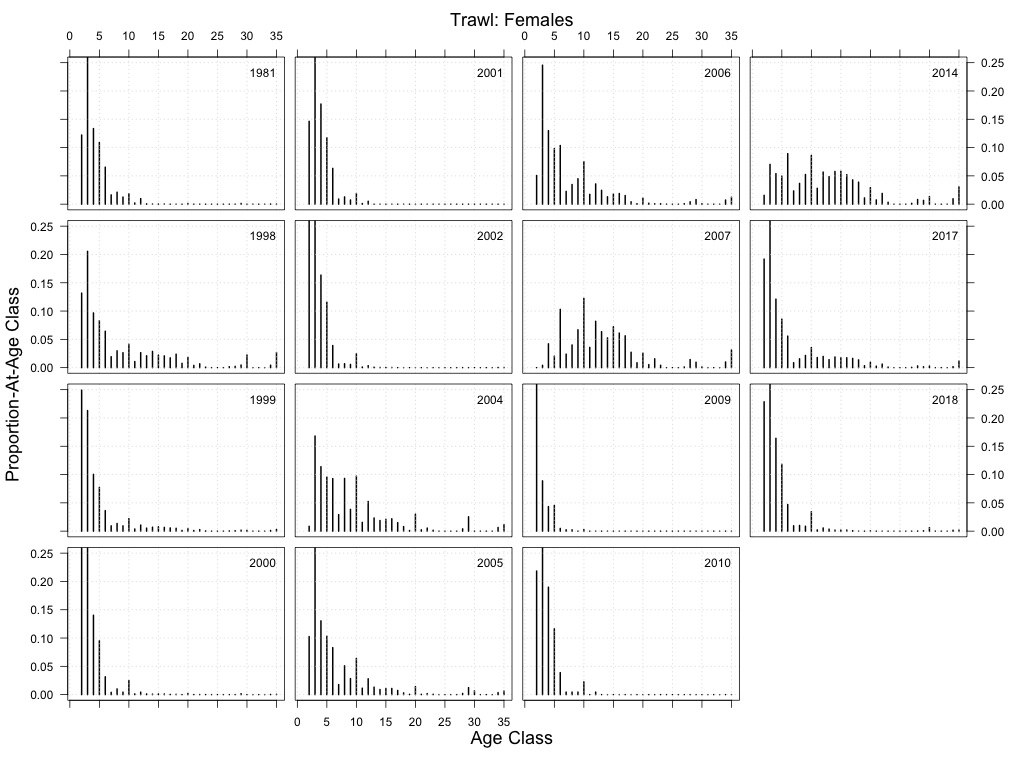
\includegraphics[width=0.9\linewidth]{data/base_ALK_mUnsexed/plotObsAgeFreq_f3}}{Figure \ref{fig:unnamed-chunk-33}} 

}

\caption{CCompositions estimées des prises femelles selon l’âge qu’a générées la clé âge-longueur de la pêche au chalut créée à partir des observations sur la longueur des poissons femelles.}\label{fig:unnamed-chunk-33}
\end{figure}
\newpage
\begin{figure}[htb]

{\centering \pdftooltip{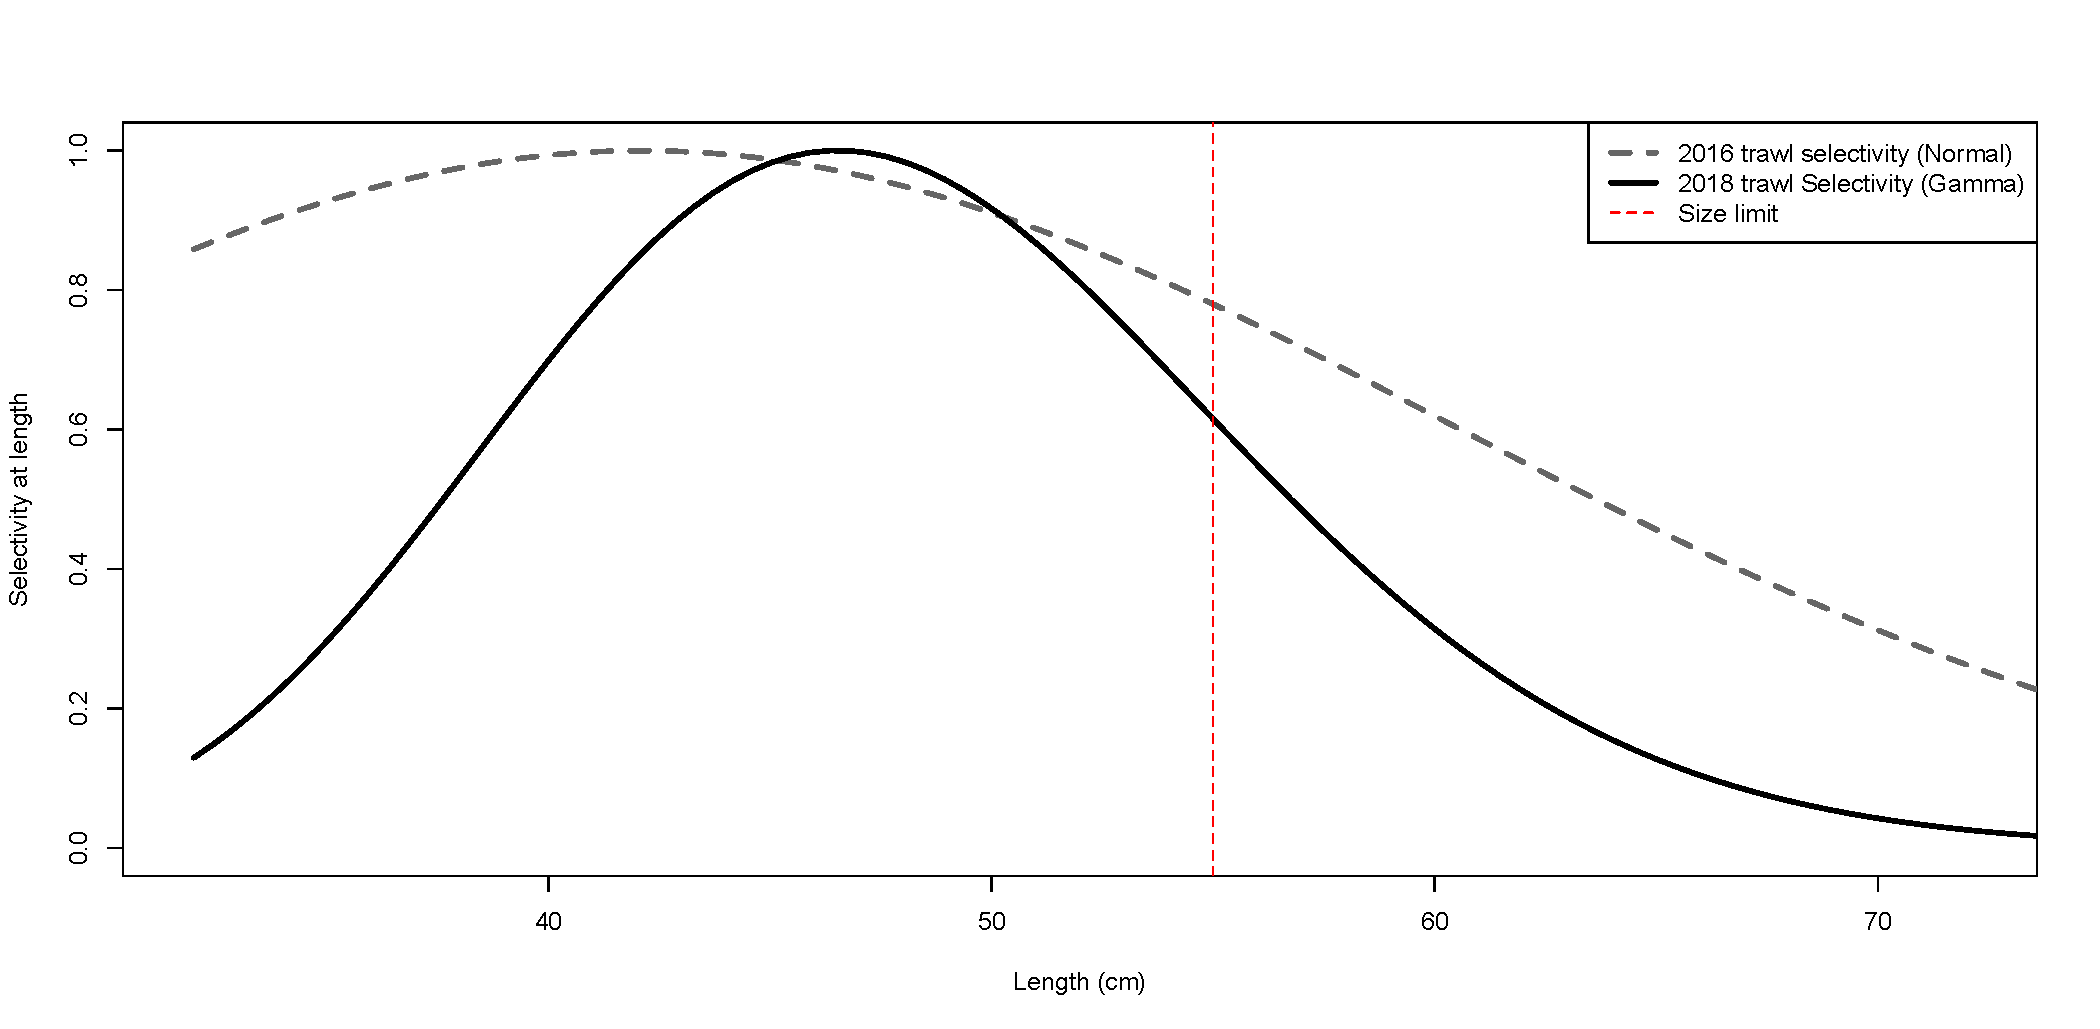
\includegraphics[width=0.9\linewidth]{data/trawlSelOverlay}}{Figure \ref{fig:unnamed-chunk-34}} 

}

\caption{Courbes de sélectivité selon la longueur pour la pêche au chalut des modèles d’exploitation de 2016 (ligne grise pointillée) et de 2019 (ligne noire pleine) et limite de taille légale (ligne pointillée rouge verticale) L’axe de longueur commence à la longueur modélisée à l’âge 1 et 32 cm.}\label{fig:unnamed-chunk-34}
\end{figure}
\clearpage

\section{Le pr\'{e}sent rapport est disponible aupr\`{e}s du}
\begin{center}
Centre des avis scientifiques\\
\rdRegion{}\\
P\^{e}ches et Oc\'{e}ans Canada\\
3190 Hammond Bay Rd.\\Nanaimo, BC, V9T 6N7\\
\vspace{0.1cm}
T\'{e}l\'{e}phone: (250) 756-7088\\
Courriel: \link{mailto:csap@dfo-mpo.gc.ca}{csap@dfo-mpo.gc.ca}\\
Addresse internet: \link{http://www.dfo-mpo.gc.ca/csas-sccs/}{www.dfo-mpo.gc.ca/csas-sccs/}\\
\vspace{0.1cm}
ISSN 1919-3769\\
\copyright{} Sa Majest\'{e} la Reine du chef du Canada, \rdYear{}\\
\vspace{0.2cm}

\includegraphics[scale=0.96]{\locRepo/images/recycle.png}
\end{center}
La pr\'{e}sente publication doit \^{e}tre cit\'{e}e comme suit:

\citeFr{\rdYear{}/\rdNumber{}}

\emph{Also available in English:}

\citeEng{\rdYear{}/\rdNumber{}}

\setlength{\parindent}{0in} \setlength{\leftskip}{0in} \setlength{\parskip}{4pt}
\hypertarget{refs}{}

\end{document}
